% concatenated from Quotient_Matrix_Revised_Nov_2025.tex
\documentclass[12pt,twoside]{article}

\usepackage{graphicx,graphics, amsthm, amsfonts, amsbsy,amssymb, amsmath, cite, array, hyperref, float,tikz,fancyvrb, hyperref,enumitem}
%\usepackage{refcheck}
\usepackage[T1]{fontenc}
\everymath{\displaystyle}
\usepackage[margin=1in]{geometry}
\usepackage{mathrsfs}
\newcommand\scalemath[2]{\scalebox{#1}{\mbox{\ensuremath{\displaystyle #2}}}}

\allowdisplaybreaks
\renewenvironment{proof}{{\noindent\bfseries Proof.}}{\qed}
%\newcommand\arrow[2]{\rotatebox{#1}{\scalebox{2}{\psline[linecolor=#2]{->}(0,0)(.03,0)}}}
\def\theequation{\thesection.\arabic{equation}}


\newtheorem{theorem}{Theorem}[section]
\newtheorem{remark}[theorem]{Remark}
\newtheorem{example}[theorem]{Example}
\newtheorem{problem}{Problem}
\newtheorem{lemma}[theorem]{Lemma}
\newtheorem{corollary}[theorem]{Corollary}
\newtheorem{definition}[theorem]{Definition}
\newtheorem{proposition}[theorem]{Proposition}
\newtheorem{note}{Note}
\newtheorem{case}{Case}
\newtheorem{conjecture}{Conjecture}
\newtheorem{question}{Question}

\usetikzlibrary{chains,positioning}
\usepackage{tikz,pgfplots}
\usetikzlibrary{decorations.pathmorphing}
% Keywords command
\providecommand{\keywords}[1]
{
	\noindent\textbf{Keywords:} #1
}
\providecommand{\ams}[2]
{
	\noindent\textbf{2020 AMS subject classification:} #2
}

\def\qed{\nolinebreak\hfill\rule{.2cm}{.2cm}\par\addvspace{.5cm}}

\linespread{1.0}
\def\hs{\hspace{.2cm}}
\begin{document}
	\title{On Matrices Whose Distinct Eigenvalues Are Fully Captured by Quotient Matrices}
	\author{
		{ Bilal Ahmad Rather$^{a}$} \\[2mm]
		\small $^{a}$School of Mathematics and Statistics, Shandong University of Technology, Zibo 255049, China\\
		$^{a}$\texttt{bilalahmadrr@gmail.com}
	}
	
	\date{}
	
	\pagestyle{myheadings} \markboth{Bilal Ahmad Rather}{On Matrices Whose Distinct Eigenvalues Are Fully Captured by Quotient Matrices}
	\maketitle
	\begin{abstract}
		Let $M$ be the $n$-square matrix partitioned into $\ell^2$ blocks $b_{ij}$ according to some partition $P=\{C_{1},\dots,C_{\ell}\}$ of index set $\{1,\dots,n\}$. The quotient matrix $Q=(q_{ij})$ is a $k$-square matrix, with $\ell \leq k \leq n-1$, where $(ij)$-th entry is the average row sum (or column sum) of the corresponding block $b_{ij}$ in $M$. The partition $P$ is said to be \emph{equitable} if row sum of each block $b_{ij}$ is constant. In this case, the matrix $Q$ is referred to as the \emph{equitable quotient matrix} of $M$, and the spectrum of $Q$ is the subset of the spectrum of parent matrix $M$. We characterize some classes of matrices such that their equitable quotient matrix $Q$ contains all the distinct eigenvalues of $M$, thereby information can be obtained form the smallest matrix $Q$ without actually analyzing the parent matrix $M.$ We present necessary and the sufficient conditions for distinct eigenvalue of $M$ contained in the spectrum of of $Q$ in terms of eigenspaces. We end up article with some applications, where distinct eigenvalues of a parent matrix can be completely encoded by quotient matrix. 
	\end{abstract}
	\vskip 3mm
	
	\keywords{Distinct Eigenvalues; Quotient Matrices; Equitable Partitions; Graph Matrices.}
	
	\ams{}{15A18, 15A42, 05C50.}

\section{Introduction}
Let $\mathcal{M}_n(\mathbb{F})$ represent the collection of all $n \times n$ matrices with entries from a field $\mathbb{F}$. For a given matrix $A \in \mathcal{M}_n(\mathbb{F})$, its collection (multiset) of eigenvalues is called the \emph{spectrum}, denoted by $\sigma(A)$. The \emph{spectral radius} of $A$, denoted $\rho(A)$, is the maximum modulus among its eigenvalues. A matrix is classified as \emph{non-negative} if every entry is non-negative. When an eigenvalue $\leftthreetimes$ as a zero of its characteristic polynomial has order $e$, then we say its algebraic multiplicity is $k$, and we employ the notation $\leftthreetimes^{[e]}$. An eigenvalue is termed as the \emph{simple} eigenvalue, if its algebraic multiplicity is one (that is, $k=1$). Our focus excludes trivial matrices such as the zero matrix, as well as diagonal and triangular matrices, whose spectral properties are straightforward and well-established. The symbol $J_{n}$ will denote the matrix whose every entry is $1$, and $I_{n}$ will represent the identity matrix of order $n.$ An indicator vector $\textbf{1}_{i}$ on a set $S$ partitioned into subsets $S_{1}\cup\dots\cup S_{t},t\geq 2$ is a vector such that its entries are $1$ for coordinates in $S_{i}$ and $0$ otherwise.
We will consider matrices in $\mathcal{M}_n(\mathbb{R}) $, where $\mathbb{R}$ is the field of of real numbers $\mathbb{R}$. 

Consider $n$-square matrix $ M_{n} $, partitioned in some block form as:
\begin{equation*}
	M= \left[ \begin{array}{c | c | c | c | c}
		b_{1,1} & b_{1,2} & \cdots & b_{1,\ell-1} & b_{1,\ell} \\
		\hline
		b_{2,1} & b_{2,2} & \cdots & b_{2,\ell-1}& b_{2,\ell} \\
		\hline
		\vdots & \vdots & \ddots & \vdots & \vdots \\
		\hline
		b_{\ell-1,1} & b_{\ell-1,2} & \cdots & b_{\ell-1,\ell-1} & b_{\ell-1,\ell}\\
		\hline
		b_{\ell,1} & b_{\ell,2} & \cdots & b_{\ell,\ell-1} & b_{\ell,\ell}\\
	\end{array}\right]_{n}. \end{equation*}
The rows and the columns of the above matrix $ M $ are partitioned according to a partition 
$P=\{ P_{1},\dots,P_{\ell}\}$ of the index set $\{1,2,\dots,n\}.$ The matrix $ Q=(q_{ij})_{\ell\times \ell}  $ with $(ij)$-th entry as the average row (or column) sum of the block $ b_{ij} $ of $ M. $ If row sum of each block $b_{ij} $ is some constant, then the partition is said to be equitable or regular, and the corresponding matrix is known as the equitable quotient matrix (see \cite{BH,heamers, cds}). For further notations or terminology about the matrices, see \cite{hj, hjl,vilmar}.

Consider two finite sequences of real numbers, $\{s_1, s_2, \dots, s_n\}$ and $\{s'_1, s'_2, \dots, s'_m\}$, where $n > m$. The sequence $\{s'_i\}$ is said to interlace the sequence $\{s_i\}$ if $s_i \geq s'_i \geq s_{n-m+i}$
holds for all $i = 1, 2, \dots, m$. This interlacing is defined as tight if there exists an integer $k$ with $0 \leq k \leq m$ such that
$$
s_i = s'_i \quad \text{for } i = 1, 2, \dots, k, \quad \text{and} \quad s_{n-m+i} = s'_i \quad \text{for } i = k+1, \dots, m.
$$
In the specific case where $m = n-1$, the general interlacing inequalities simplify to the classic, chain-like form:
$$
s_1 \geq s'_1 \geq s_2 \geq s'_2 \geq \cdots \geq s_{n-1} \geq s'_{n-1} \geq s_n.
$$

The paper is organized as: In section \ref{section 2}, we discuss some existing results and present some new classes of matrices such that their quotient matrix containing distinct eigenvalues of $M.$ In Section \ref{section 3}, we characterize matrices such that quotient matrix contains the two distinct eigenvalue of matrix $M.$ Section \ref{section 5}, investigates the distinct eigenvalues of quotient matrices of graph matrices Section \ref{section 6}, presents results related to the quotient matrix which contains all the distinct eigenvalues of the Laplacian matrices assigned to graphs.

\section{Quotient matrix containing all the distinct eigenvalues of matrix $M$}\label{section 2}
In this section, we recall some basic existing results and present some new results related to the distinct eigenvalues of the quotient matrix of parent matrix $M.$ In Section \ref{section 4}, we discuss the necessary and the sufficient condition for the matrix $M$ with some equitable partition $\pi$ such that its quotient matrix contains all the distinct eigenvalues. 

The following result gives the relation between the eigenvalues of $ M $ and the eigenvalues of $ Q. $
\begin{lemma}[\cite{heamers}]\label{quotient matrix eigenvalues}
	Let $ M $ be a real symmetric matrix of order $ n $ and $ Q $ be its quotient matrix. Then the following hold.
	\begin{enumerate}
		\item If the partition $ P $ of $ I$ of matrix $ M $ is not equitable, then eigenvalues of $ Q $ interlace the eigenvalues of $ M $.
		\item If the partition $ P $ of $ I $ of matrix $ M $ is equitable, then the interlacing is tight, that is, the spectrum of $ Q $ is the subset of the spectrum of $ M. $
	\end{enumerate}
\end{lemma}


Quotient matrices are very important matrices associated to parent matrices related to some partitions. These matrices have many applications in the spectral theory of graph matrices. In case partition is not equitable, then we can find bounds for the eigenvalues of the original matrix due to their interlacing fact. In case the partition is equitable then we get some information about the spectrum of the original matrix. Some of the applications and the properties of quotient matrices can be seen in \cite{DS, mehreen1, atikELA2018, you,bilal2020, bilal}. Our motivation is that: is it possible to find all the information about the spectrum of original matrix $ M$ form its smallest possible equitable quotient matrix.  A similar idea about the spectral radius of parent matrix $M$ and its quotient matrix $Q.$ We have a partial answer for non-negative matrices, in tersm of the following result.
\begin{lemma}[\cite{atikELA2018, you}]\label{spectral radius of positive matrices}
	The spectral radius of a non-negative matrix $ M $ and the spectral radius of an equitable quotient matrix $ Q $ coincide.
\end{lemma}
For matrices with negative entries, Lemma \ref{spectral radius of positive matrices} fails, as can be seen below:
 $$M=\left[
\begin{array}{cccc}
	10 & -1 & -1 & -4 \\
	-1 & 10 & -1 & -4 \\
	6 & 6 & -14 & 1 \\
	6 & 6 & 1 & -14 \\
\end{array}
\right].
$$
The spectrum of $M$ is $ \{11,5.81025, -15, -9.81025\}$. The quotient matrix with equitable partition  $\{\{1,2\},\{3,4\}\} $ is	$ 	m=\left[
\begin{array}{cc}
	9 & -5 \\
	12 & -13 \\
\end{array}
\right],
$  and the spectrum of $M$ is $	\{5.81025, -9.81025\}$. Thus $M$ and its associated equitable quotient matrix does not share the same spectral radius for completely non-positive matrices. More counterexamples can be seen in \cite{atikELA2018, you, bilalijpam}. Motivated by Lemma \ref{spectral radius of positive matrices}, how about the other eigenvalues of $M$? When does $M$ and $Q$ share all the distinct eigenvalues. 
More formally, if the spectrum of $M$ is $ \{\leftthreetimes_{1}^{n_{1}},\leftthreetimes_{2}^{n_{2}},\dots, \leftthreetimes_{t}^{n_{t}}\},$ are the distinct eigenvalues of $ M $, then is it true that $ \leftthreetimes_{1},\leftthreetimes_{2},\dots, \leftthreetimes_{t} $ are always the eigenvalues of $ Q $, $ t\geq 2, n_{i}\geq 1 $ and $\sum_{i=1}^{t}n_{i}=n$. In this regard, Atik \cite{atik} asked the following problem about the distinct eigenvalues of the equitable quotient matrix of  $ M $.
\begin{problem}[Atik, \cite{atik}]\label{distinct eigenvalue problem}
	What is the necessary and sufficient condition on the equitable quotient matrix $ Q $ to contain all the distinct eigenvalues of $ M $?
\end{problem}

Problem \ref{distinct eigenvalue problem} was studied rigorously in \cite{bilalijpam}, the significant observation was that: it is a problem related to  equitable partitions, with one partition $Q$ and $M$ will share same distinct eigenvalues but with another partition property of distinct eigenvalues may fail. The problem was restated about the smallest equitable possible partition so that from the quotient matrix $Q$, we can encode all the distinct eigenvalues of the parent matrix $M.$ The following grantee for such a equitable partitions. 
\begin{theorem}[\cite{bilalijpam}]\label{theorem eqitable quotient matrix contains all the eigenvalues with some partition}
	Let $ M $ be a matrix of order $ n $ and $ Q $ be its equitable quotient matrix. Then the following holds.
	\begin{enumerate}
		\item There exists an equitable partition such that its quotient matrix $ Q $ contains the spectral radius of $ M. $
		\item There exists an equitable partition such that its quotient matrix $ Q $ contains all the distinct eigenvalues of $ M. $
	\end{enumerate}
\end{theorem}

Related to the distinct eigenvalue of equitable quotient $Q$ and the parent matrix $M,$ the following problem was asked in \cite{bilalijpam}.
\begin{problem}\label{problem distinct 2}
	Characterize those matrices such that the spectrum of the quotient matrix contains all the distinct eigenvalues of parent matrix with respect to the smallest equitable partition?
\end{problem}



Related to Problem \ref{problem distinct 2}, the following class of the matrices was given in \cite{bilalijpam}, such that its equitable quotinet matrix contains all the distinct eigenvalues with respect to the smallest partition $P=\{\{1\},\{2\},\{3,\dots,n+2\}\}.$
\begin{proposition}\label{Qmat contains distinct eigenvalues of M}
	Let $ M $ be the matrix given as
	\begin{equation}\label{matrix containing all distinct eigenvalues}
		M=\left[ \begin{array}{c | c | c c c c c}
			4n-2 & -(2n-2) & -2   & -2 & \dots   & -2 & -2\\
			\hline
			-1   & 4n+1   & -4   & -4 & \dots   & -4 & -4\\
			\hline
			-1   & -2(2n-2) & 8n-7 & -4 & \dots   & -4 & -4\\
			-1   & -2(2n-2) & -4 & 8n-7 & \dots   & -4 & -4\\
			\vdots & \vdots & \vdots & \vdots & \ddots & \vdots & \vdots\\
			-1   & -2(2n-2) & -4 & -4 & \dots   & 8n-7 & -4\\
			-1   & -2(2n-2) & -4 & -4 & \dots   & -4 & 8n-7
		\end{array}
		\right ]_{n+2}. 
	\end{equation}
	 Then it's equitable quotient matrix $ Q $ given in \eqref{Qmat of special M} contains all the distinct eigenvalues of $ M. $
	\begin{equation}\label{Qmat of special M}
		Q=\begin{bmatrix}
			4n-2 & -(2n-2) & -2n\\
			-1   & 4n+1    & -4n\\
			-1   & -2(2n-2)& 4n-3
		\end{bmatrix}.
	\end{equation}
\end{proposition}
Several interesting results related to \ref{distinct eigenvalue problem} were given in \cite{bilalijpam}; notably identifying the problem about partitions, result related to enlarging partition (Theorem 2.7 \cite{bilalijpam}), classes of matrices such that their equitable quotient matrix with smallest partition containing arbitrary number of distinct eigenvalues of parent matrix except one eigenvalue (Theorem 2.6 \cite{bilalijpam}), and other illustrations. We have technical refinement about Proposition \ref{Qmat contains distinct eigenvalues of M}, the matrix given in \eqref{Qmat of special M} is not the smallest equitable possible quotient matrix, rather it is the second smallest equitable quotient matrix which contains all the distinct eigenvalue of matrix given in \eqref{matrix containing all distinct eigenvalues}. As the smallest equitable quotient matrix of \eqref{matrix containing all distinct eigenvalues} is the matrix $Q=(0)_{1\times 1}$ with partition $P=\{1,2,\dots,n+2\}$. It contains only one eigenvalue with the smallest equitable partition. \vskip 2mm

Thus, we are still searching  for a matrix $M$ such that its equitable matrix $Q$ contains all the distinct eigenvalues, and that will partially answer Problem \eqref{problem distinct 2}.

Consider the matrix $M$ of order $n$,  given below
\begin{equation}\label{mat 1}
	 M=\begin{bmatrix}
	1 & -aJ_{1\times (n-1)}\\
	a J_{(n-1)\times 1} & bI_{n-1}+a(J_{n-1}-I_{n-1})
\end{bmatrix}_{n},
\end{equation}
where $a$ and $b$ are scalers. The matrix has positive as well as negative entries. Consider the following vectors
\begin{align*}
	X_{1}&=(0,-1,0,\dots,0,1),X_{2}=(0,-1,0,\dots,1,0), X_{3}=(0,-1,0,\dots,0,1,0,0),\\
	&\vdots\\
	X_{n-3}&=(0,-1,0,0,1,0,\dots,0, 0), X_{n-2}=(0,-1,0,1,0,\dots,0,0),X_{n-1}=(0,-1,1,0,\dots,0).
\end{align*} 
Each of these vectors are trivially linearly independent, and $MX_{i}^{T}=(b-a)X_{i}^{T}$, for $i=1,2,\dots,n-1$. Now, consider the partition $P=\{\{1,2,\dots,n\}\}$, then its quotient matrix is not equitable as first row sum is  $1-(n-1)a$ and second row sum is $b+(n-1)a$, which are not equal in general. The quotient matrix is inequitable. Consider the partition \( P=\{\{1\},\{2,3,\dots,n\}\} \), with the corresponding quotient matrix given by $$Q=\begin{bmatrix} 1 & -(n-1)a\\ (n-1)a & b+(n-2)a \end{bmatrix}.$$
The eigenvalues of \( Q \) are $$ \frac{1}{2} \left(a n - 2 a + b + 1 \pm \sqrt{(a (-n) + 2 a - b - 1)^2 - 4 \left(a^2 n - a^2 + a n - 2 a + b\right)}\right). $$Consequently, it follows that $P=\{\{1\},\{2,3,\dots,n\}\}$ represents the minimal equitable partition and does not encompass all distinct eigenvalues of $M$, as the eigenvalue $b-a$ is absent. 


We will refine the matrix \( M \) as presented in \eqref{mat 1} with \( a=2 \) and \( b=7 \), and define $$ M^{\prime}=\begin{bmatrix} 1 & -2J_{1\times (n-1)}\\ 2 J_{(n-1)\times 1} & 5I_{n-1}+2(J_{n-1}-I_{n-1}) \end{bmatrix}_{n\times n}. $$
Let \( X = (-1, 1, \ldots, 1) \) denote a vector. Consequently, $M^{\prime}X^{T}=(2n-1)X^{T}$, where $X^{T}$ denotes the transpose of $X$. Thus, $2n-1$ is an eigenvalue of $M^{\prime}$ corresponding to the eigenvector $X$. Similarly, for matrix $M^{\prime}$ in \eqref{mat 1}, we obtain $M^{\prime}X_{i}^{T}=3X_{i}^{T}$, for $i=1,2,\dots,n-1$. Consequently, the spectrum of $M^{\prime}$ is $\{2n-1,3^{n-1}\}$. Consequently, $M^{\prime}$ possesses two unique eigenvalues. Consider the partition \( P=\left \{\{1,2,\dots,n\}\right \} \). It is evident that \( M \) lacks a constant row sum, so \( P \) does not constitute an equitable partition. Next, examine an alternative partition $P^{\prime}=\left \{\{1\},\{2,3,\dots,n\}\right \}$. Then $P^{\prime}$ is equitable partition as $M^{\prime}$ has constant row sums in respective blocks. The equitable quotient matrix is 
$$ Q^{\prime}=\left[
\begin{array}{cc}
	1 & -2 (n-1) \\
	2 & 2 (n-2)+5 \\
\end{array}
\right].$$
The eigenvalues of $Q$ are $\{3,2n-1\}.$ Thus for the matrix $M^{\prime}$ and with the smallest equitable partition $P^{\prime}=\left \{\{1\},\{2,3,\dots,n\}\right \}$, its quotient matrix $Q^{\prime}$  contains all the distinct eigenvalues of matrix $M^{\prime}$. If you choose any other partition with two cell and one cell as singleton, then matrix $Q$ is not equitable. Like choose $P^{''}=\left \{\{1,2,\dots,n-1\},\{n\}\right \}$, then its associated quotient matrix is not equitable as last block does not have constant row sum. Thus, we have a class of matrix $M^{\prime}$ which satisfies the requirement of Problem \ref{problem distinct 2}. We make it precise in the following result.
\begin{proposition}
	Let $M_{n}$ be a matrix defined as
	$$ M=\begin{bmatrix}
		1 & -2J_{1\times (n-1)}\\
		2 J_{(n-1)\times 1} & 5I_{n-1}+2(J_{n-1}-I_{n-1})
	\end{bmatrix}_{n\times n}. $$
	Then  with the smallest equitable partition $P=\{\{1\},\{2,3,\dots,n\}\}$, its equitable quotient matrix $Q$ contains all the distinct eigenvalues of $M,$ where
	$$ Q^{\prime}=\left[
	\begin{array}{cc}
		1 & -2 (n-1) \\
		2 & 2 (n-2)+5 \\
	\end{array}
	\right].$$
\end{proposition}

Consider another matrix defined as
$$M=\begin{bmatrix}
	\frac{1}{\alpha}J_{a} & J_{a\times b}\\
	J_{b\times a} & \alpha J_{b}
\end{bmatrix}_{a+b},$$ where $\alpha$ is real and $a,b$ are positive integers. Choose
$$X_{i}=(-a,x_{2i}, x_{3i},\dots,x_{(a+b)i}), \quad i=2,\dots,a+b,$$ where $x_{i}=\delta_{ij}$, where $ \delta_{ij}$ is Kronecker delta function. Then it is easy to see that $X_{i}$'s are the eigenvector of $M$ with related eigenvalue $0.$ So, $0$ is the eigenvalue of $M$ with multiplicity $a+b-1.$ Also, by choosing $X=\Big(\underbrace{\frac{1}{a},\dots,\frac{1}{a}}_{a},\underbrace{1,1,\dots,1}_{b}\Big)$, and evaluating $MX^{t}$, we get $\left(\frac{a+\alpha ^2 b}{\alpha }\right)X^{t}.$ It follows that $ \frac{a+\alpha ^2 b}{\alpha }$ is the simple eigenvalue of $M.$ Clearly, $M$ has no equitable quotient matrix with partition $\{1,2,\dots,a,a+1,\dots,a+b\}. $ Next, if we choose partition $P=\{\{1,2,\dots,a\},\{a+1,\dots,a+b\}\}$, we have the equitable quotient matrix $Q=\left[\begin{array}{cc}
	\frac{a}{\alpha } & b \\
	a & \alpha  b \\
\end{array}
\right],$ and its eigenvalues are $\left\{0,\frac{a+\alpha ^2 b}{\alpha }\right\}.$ So, $M$ is another class of matrices such that its equitable quotient matrix contains all the distinct eigenvalue of $M$ with the smallest possible equitable partition. Characterising all such matrices and answering Problem \ref{problem distinct 2} is very non trivial. However, even finding a one class of matrices is worth and it gives us positive hope for the partial solution of Problem \ref{problem distinct 2}.\vskip 2mm

For matrix of order $1$, that is, $M=(a)_{1}$, there is noting to prove. For $M=\begin{bmatrix}
	a & b\\
	c & d
\end{bmatrix},$ if $\leftthreetimes_{1}\neq \leftthreetimes_{2}$ are two distinct eigenvalues of $M$, there is noting to prove. Now, if $\leftthreetimes_{1} = 0, $ or $\leftthreetimes_{2}=0$, the matrix $M$ is itself the quotient matrix of order $2.$ For $\leftthreetimes_{1}=\leftthreetimes_{2}$, we get $$ (a-d)^{2}+4bc=0. $$
If $b = 0$, then $(a - d)^2 + 0 = 0  $ implies that $ a = d$ and $c$ can be anything.  For any $a, b,$ we can choose $d = a$ and $c = 0,$ 
then the eigenvalues are $a, a$. A similar situation works for $d=a$ and $b=0.$  And in that case $M$ is itself quotient matrix with the smallest possible partition $\{\{1,2\}\}$. 

Next for $3\times 3$ matrices, we consider 
$$M= \left[ \begin{array}{ccc} m_{11} & m_{12} & m_{13} \\  m_{21} & m_{22} & m_{23} \\ m_{31} & m_{32} & m_{33} \end{array} \right]. $$
If $M$ has three distinct eigenvalues, then we have to do nothing as in this case $Q$ is itself $M$. Also, $M$ can have only one eigenvalues if it is zero, scalar or triangular matrix with same diagonal entries, which we ignore due to their trivial behaviour. Assume that there is an eigenvalue $\leftthreetimes$ with multiplicity $2,$ and write $M$ in the form  
$$ M= \left[ \begin{array}{c|cc} m_{11} & m_{12} & m_{13} \\ \hline m_{21} & m_{22} & m_{23} \\ m_{31} & m_{32} & m_{33} \end{array} \right],$$
where partition is $P=\{\{1\},\{2,3\}\}.$ For this partition to be equitable, the row sums of each block must be constant. Let these constant sums be $c_{ij}$. The equitable quotient matrix is \begin{equation}\label{qmatt}
	Q = \begin{bmatrix} c_{11} & c_{12} \\ c_{21} & c_{22} \end{bmatrix},
\end{equation}
where \begin{align}\label{system eq 1}
 m_{11} = c_{11}, m_{12} + m_{13} = c_{12}, m_{21} = m_{31} = c_{21}, m_{22} + m_{23} = m_{32} + m_{33} = c_{22}.
\end{align}
In this case, each eigenvalues of $Q$ is the eigenvalues of $M$. Let $\alpha\leq \beta$ be the two real distinct eigenvalues of $Q.$ We need to modify entries of $M$ such that one eigenvalue say $\alpha$ is the repeated eigenvalue of $M.$ The eigenvector of $M$ corresponding to $\leftthreetimes_3$ must lie in the subspace orthogonal to the subspace of vectors that are constant on the cells of the partition. For our partition, this subspace is spanned by the vector $X= (0, 1, -1)^t$. Let us modify $M$ such that $X$ is an eigenvector with eigenvalue $\leftthreetimes_3= \alpha$. By evaluation $MX=\alpha X,$ we have 
\begin{equation}\label{system eq 2}
	m_{12}-m_{13}=0, m_{22}-m_{23}=\alpha, m_{32}-m_{33}=-\alpha.
\end{equation}
By comparing the system of equations in \eqref{system eq 1} and \eqref{system eq 2}, and after solving, we have
\begin{align*}
	m_{12}=m_{13}=\frac{c_{12}}{2}, m_{22}=m_{33}=\frac{c_{22}+\alpha}{2}, m_{23}=m_{32}=\frac{c_{22}-\alpha}{2}.
\end{align*}
Thus, $M$ can be written as 
\begin{equation}\label{qmat 3}
	M=\left[
\begin{array}{ccc}
	c_{11} & \frac{c_{12}}{2} & \frac{c_{12}}{2} \\
	c_{21} & \frac{1}{2} \left(\alpha+c_{22}\right) & \frac{1}{2} \left(c_{22}-\alpha\right) \\~\\
	c_{21} & \frac{1}{2} \left(c_{22}-\alpha\right) & \frac{1}{2} \left(\alpha+c_{22}\right) \\
\end{array}
\right].
\end{equation}
So for $3\time 3$ matrix $M$ given as above, the smallest equitable quotient matrix $Q$ given in \eqref{qmatt} contains all the distinct eigenvalues of $M.$ This solves the problem of distinct eigenvalues in equitable quotient matrix of matrices of order $1,2,$ and $3.$

Lets us illustrate the above fact with the help of the example. Choosing $Q$ as given below
$$ Q = \begin{bmatrix} 1 & -8 \\ 4 & 13 \end{bmatrix} .$$
The eigenvalues of $Q$ are $\{5,9\}$. For $\alpha=5$ with $c_{11}=1,c_{12}=-8,c_{21}=4$ and $c_{22}=13,$ we have
$$M=\left[
\begin{array}{ccc}
	1 & -4 & -4 \\
	4 & 9 & 4 \\
	4 & 4 & 9 \\
\end{array}
\right],$$
and its eigenvalues are $\{5^{2},9\}$. Thus, $Q$ is the smallest possible equitable matrix which contains all the distinct eigenvalues of $M.$

To check for uniqueness, consider the other two partitions of size $2$ with cell sizes $P_{1}=\{\{1,3\},\{2\}\}$ and $P_{2}=\{ \{1,2\},\{3\}\}$.
For $P_{2}$, the row sum of first block is $-3, $ and $13$, which are not constant, and $P_{2}$ is not equitable. Similarly, row sum quotient matrix for the partition $P_{1}$ are not constant, and its quotient matrix  is not equitable. Thus, we have only $\binom{3}{2}=3$ partitions with two cell. The only equitable partition is $\{\{1\},\{2,3\}\}$, and its equitable quotient matrix contains all the distinct eigenvalues of $M.$ This, idea can be generalized to matrices of order $4, 5,6$ and so on. It may be hard for matrices of larger order but it is interesting to construct their representations as in \eqref{qmat 3}, and that will contribute to Problem \ref{problem distinct 2}.


\section{Characterization of matrices with two distinct eigenvalues in quotient matrix}\label{section 3}
Generalizing the above idea for the square matrices of order $4$. Consider the following matrix with partition $\pi=\bigl\{\{1\},\{2,3,4\}\bigr\}$
	$$
	M=\left[ \begin{array}{c|ccc}
		m_{11} & m_{12} & m_{13} & m_{14}\\
		\hline
		m_{21} & m_{22} & m_{23} & m_{24}\\
		m_{31} & m_{32} & m_{33} & m_{34}\\
		m_{41} & m_{42} & m_{43} & m_{44}
	\end{array}\right].
	$$
 The partition $\pi$ is equitable for $M$ if and only if the row sums of each
	block are constant. Let these constants be $c_{ij}$, so that the equitable
	quotient matrix is
	\begin{equation}\label{eq:Q-4x4}
		Q=
		\begin{bmatrix}
			c_{11} & c_{12}\\
			c_{21} & c_{22}
		\end{bmatrix},
	\end{equation}
	where
	\begin{equation}\label{eq:system-1-4x4}
		\begin{aligned}
			m_{11}=c_{11}, m_{21}=m_{31}=m_{41}=c_{21},\\
				m_{22}+m_{23}+m_{24}=c_{22},m_{32}+m_{33}+m_{34}=c_{22},\\
				m_{42}+m_{43}+m_{44}=c_{22}, m_{12}+m_{13}+m_{14}=c_{12}
		\end{aligned}
	\end{equation}
	As $\pi$ is equitable, so each eigenvalue of $Q$ is an eigenvalue of $M$.	Let $\alpha<\beta$ be the two real distinct eigenvalues of $Q$. 	We now seek a $4\times 4$ matrix $M$ with only these two distinct
	eigenvalues, such that $\operatorname{spec}(M)=\{\alpha^{3},\beta\},$ 	and $\pi$ is an equitable partition whose quotient $Q$ contains both eigenvalues
	$\alpha,\beta$.  The partition subspace of vectors constant on the cells of $\pi$ is
	$$
	W=\{(a,b,b,b)^{\mathsf T}: a,b\in\mathbb{R}\}\subset\mathbb{R}^4,
	$$
	spanned by $e_1=(1,0,0,0)^{\mathsf T}$ and $u=(0,1,1,1)^{\mathsf T}$. Its
	orthogonal complement (with respect to the standard inner product) is
	$$
	W^\perp
	=
	\{(0,y,z,w)^{\mathsf T}: y+z+w=0\},
	$$
	which is $2$--dimensional. A convenient basis of $W^\perp$ is
	$$
	X_1=(0,1,-1,0)^{\mathsf T},\qquad
	X_2=(0,1,0,-1)^{\mathsf T}.
	$$
	To make $\alpha$ the repeated (triple) eigenvalue of $M$, we require that
	$W^\perp$ be contained in the eigenspace of $\alpha$, that is, we impose
	$$
	M X_1 = \alpha X_1,
	\qquad
	M X_2 = \alpha X_2.
	$$
	
	A direct computations from $M X_1=\alpha X_1$ and $M X_2=\alpha X_2$
	$$
		m_{12}-m_{13}=0,		m_{22}-m_{23}=\alpha,
		m_{32}-m_{33}=-\alpha,		m_{42}-m_{43}=0,
	$$
	and
	$$
		m_{12}-m_{14}=0,
		m_{22}-m_{24}=\alpha,
		m_{32}-m_{34}=0,
		m_{42}-m_{44}=-\alpha.
	$$
	Combining the above two equations with the equitability conditions given in	\eqref{eq:system-1-4x4}, we obtain
	$$
	m_{12}=m_{13}=m_{14}=\frac{c_{12}}{3}, \quad \text{and}\quad m_{21}=m_{31}=m_{41}=c_{21}.
	$$
	With these values, the $3\times 3$ block $B=(m_{ij})_{2\le i,j\le 4}$ in $M$ has the form
	\begin{equation}\label{eq:B-structure}
		B
		=
		\frac{1}{3}
		\begin{bmatrix}
			2\alpha + c_{22} & -\alpha + c_{22} & -\alpha + c_{22}\\
			-\alpha + c_{22} & 2\alpha + c_{22} & -\alpha + c_{22}\\
			-\alpha + c_{22} & -\alpha + c_{22} & 2\alpha + c_{22}
		\end{bmatrix}
		=
		\alpha I_3 + \frac{c_{22}-\alpha}{3}J_3,
	\end{equation}
	where $J_3$ is the $3\times 3$ all--ones matrix.
	Thus, the matrix $M$ can be written as
	\begin{equation}\label{eq:M-4x4-final}
		M
		=
		\begin{bmatrix}
			c_{11} & \frac{c_{12}}{3} & \frac{c_{12}}{3} & \frac{c_{12}}{3}\\
			c_{21} & \frac{2\alpha+c_{22}}{3} & \frac{c_{22}-\alpha}{3} & \frac{c_{22}-\alpha}{3}\\
			c_{21} & \frac{c_{22}-\alpha}{3} & \frac{2\alpha+c_{22}}{3} & \frac{c_{22}-\alpha}{3}\\
			c_{21} & \frac{c_{22}-\alpha}{3} & \frac{c_{22}-\alpha}{3} & \frac{2\alpha+c_{22}}{3}
		\end{bmatrix}.
	\end{equation}
	
	As the partition $\pi$ is equitable with quotient $Q$ given  in
	\eqref{eq:Q-4x4}, so the matrix $M$ leaves $W$ invariant, and the restriction
	$M|_W$ has matrix $Q$ in the basis $\{e_1,u\}$. Thus, the eigenvalues of $Q$,
	namely $\alpha$ and $\beta$, are eigenvalues of $M$ with eigenvectors in $W$. Also, the $3\times 3$ block $B$ in \eqref{eq:B-structure} satisfies
	$$
	B x = \alpha x
	\quad\text{for all }x\in\mathbb{R}^3\text{ with }x_1+x_2+x_3=0,
	$$
	since $J_3x=0$ in that case. This is exactly the image of $W^\perp$ under the
	projection onto the last three coordinates, and we have explicitly arranged $M X_1=\alpha X_1,$ and $M X_2=\alpha X_2,$	so that $W^\perp\subseteq E_\alpha$ with $\dim W^\perp=2$.
	Therefore,  $M|_W$ has eigenvalues $\alpha$ and $\beta$ (one eigenvector for each in $W$), and   $M|_{W^\perp}$ is $\alpha I$ (two independent eigenvectors in $W^\perp$).
	Hence,  $\operatorname{spec}(M)=\{\alpha^{3},\beta\},$ and $\alpha,\beta$ are precisely the eigenvalues of the smallest equitable quotient matrix $Q$, of order $2$.   Let us illustrate the above fact with the help of an example.  Consider the matrix 
	$Q=
	\begin{bmatrix}
		1 & 0\\
		3 & 4
	\end{bmatrix}.$ The eigenvalues of $Q$ are $\{1,4\}.$ We choose $\alpha=1$, the eigenvalue that will be repeated in $M$ and $\beta=4$, the simple eigenvalue of $M$. With the above notations, $	c_{11}=1,\quad c_{12}=0,\quad c_{21}=3,\quad c_{22}=4.$ Now, we construct $M$ from $Q$ and $\alpha$. Thus, we have
	$$
	M
	=
	\begin{bmatrix}
		c_{11} & \dfrac{c_{12}}{3} & \dfrac{c_{12}}{3} & \dfrac{c_{12}}{3}\\
		c_{21} & \dfrac{2\alpha+c_{22}}{3} & \dfrac{c_{22}-\alpha}{3} & \dfrac{c_{22}-\alpha}{3}\\
		c_{21} & \dfrac{c_{22}-\alpha}{3} & \dfrac{2\alpha+c_{22}}{3} & \dfrac{c_{22}-\alpha}{3}\\
		c_{21} & \dfrac{c_{22}-\alpha}{3} & \dfrac{c_{22}-\alpha}{3} & \dfrac{2\alpha+c_{22}}{3}
	\end{bmatrix},
	$$
	with $\alpha=1$, $c_{11}=1$, $c_{12}=0$, $c_{21}=3$, $c_{22}=4$, we obtain
	$$
	\frac{c_{12}}{3}=0,\quad
	\frac{2\alpha+c_{22}}{3}=\frac{2\cdot 1+4}{3}=2,\quad
	\frac{c_{22}-\alpha}{3}=\frac{4-1}{3}=1.
	$$
	Thus, the matrix $M$ is
	$$
	M
	=
	\begin{bmatrix}
		1 & 0 & 0 & 0\\
		3 & 2 & 1 & 1\\
		3 & 1 & 2 & 1\\
		3 & 1 & 1 & 2
	\end{bmatrix}.
	$$
Clearly, $Q$ is its equitable quotient matrix with partition $\pi=\bigl\{\{1\},\{2,3,4\}\bigr\},$ and the eigenvalues of $Q$ are $1$ and $4$. We now show that $1$ has multiplicity $3$ and $4$ has multiplicity $1$. The partition subspace
	$$
	W = \{(a,b,b,b)^{\mathsf T}: a,b\in\mathbb{R}\}
	= \operatorname{span}\{e_1,\;u\},
	\quad
	u=(0,1,1,1)^{\mathsf T},
	$$
	is $M$-invariant and on $W$ the matrix of $M$ (in the basis $\{e_1,u\}$) is
	exactly $Q$. Thus, $M$ has eigenvectors in $W$ for eigenvalues $1$ and $4$. For $\leftthreetimes=4$, an eigenvector of $Q$ is $(0,1)^{\mathsf T}$, giving the
	eigenvector $u=(0,1,1,1)^{\mathsf T}$	of $M$ with $M u = 4u.$ For $\leftthreetimes=1$, an eigenvector of $Q$ is $(1,-1)^{\mathsf T}$, giving $x_W = e_1 - u = (1,-1,-1,-1)^{\mathsf T},$	and $M x_W = x_W.$ So,  $x_W$ is an eigenvector of $M$ with eigenvalue $1$ lying in $W$.  The orthogonal complement of \( W \) is $$ W^\perp = \{(0,y,z,w)^{\mathsf T} : y+z+w=0\}. $$ The space is spanned by \(X_1 = (0,1,-1,0)^{\mathsf T}\) and \(X_2 = (0,1,0,-1)^{\mathsf T}\). A straightforward computation reveals that \(M X_1 = X_1\) and \(M X_2 = X_2\), indicating that \(X_1\) and \(X_2\) are eigenvectors of \(M\) corresponding to the eigenvalue \(1\), and they are orthogonal to \(W\). 
	 Thus, for the matrix $M$,  one eigenvector $u$ for the eigenvalue  $\leftthreetimes=4$, and three linearly independent eigenvectors $x_W,\;X_1,\;X_2$ for the eigenvalue $\leftthreetimes=1$.  So, the spectrum of $M$ is  $\{1^3,4\}$, and the smallest equitable quotient matrix $Q$  contains all distinct eigenvalues $1$ and $4$ of $M$.

The second possibility for the spectrum of $M$ is $\{\alpha^{[2]},\beta^{[2]}\}.$ We need to find $Q$ with smallest possible partition such that it spectrum is $\{\alpha,\beta\}.$ We consider this case in the following theorem.
\begin{theorem}\label{thm:4x4-two-eigs}
	Let $Q$ be a real $2\times 2$ matrix $Q=
	\begin{bmatrix}
		c_{11} & c_{12}\\
		c_{21} & c_{22}
	\end{bmatrix},$ 	with two distinct real eigenvalues $\sigma(Q)=\{\alpha,\beta\},$ with $ \alpha\neq\beta.$
	Define the $4\times 4$ matrix $M$ (depending on $Q,\alpha,\beta$) by
	\begin{equation}\label{eq:M-4x4}
		M=
		\begin{bmatrix}
			\displaystyle \frac{c_{11}+\alpha}{2} & \displaystyle \frac{c_{11}-\alpha}{2} & \displaystyle \frac{c_{12}}{2} & \displaystyle \frac{c_{12}}{2}\\
			\displaystyle \frac{c_{11}-\alpha}{2} & \displaystyle \frac{c_{11}+\alpha}{2} & \displaystyle \frac{c_{12}}{2} & \displaystyle \frac{c_{12}}{2}\\
			\displaystyle \frac{c_{21}}{2} & \displaystyle \frac{c_{21}}{2} & \displaystyle \frac{c_{22}+\beta}{2} & \displaystyle \frac{c_{22}-\beta}{2}\\
			\displaystyle \frac{c_{21}}{2} & \displaystyle \frac{c_{21}}{2} & \displaystyle \frac{c_{22}-\beta}{2} & \displaystyle \frac{c_{22}+\beta}{2}
		\end{bmatrix}.
	\end{equation}
	Then $Q$ contains both the distinct eigenvalues of $M$ with the smallest equitable partition  $\pi=\bigl\{\{1,2\},\{3,4\}\bigr\}.$
\end{theorem}
\begin{proof}
	Let $M$ be the matrix of order $4,$ and $\pi=\{\{1,2\},\{3,4\}\}$ be the equitable partition with corresponding quotient matrix $Q$. 	The characteristic matrix of the partition $\pi=\{\{1,2\},\{3,4\}\}$ is  $P=
	\begin{bmatrix}
		1 & 0\\
		1 & 0\\
		0 & 1\\
		0 & 1
	\end{bmatrix},$	whose columns span the subspace of the vectors constant on each cell
	$$
	W = \operatorname{im}P
	=
	\{(a,a,b,b)^\mathsf{T} : a,b\in\mathbb{C}\}.
	$$
	The equitable quotient \( Q \) is defined by the equationM P equals P Q.The sum of the elements in row $1$ and row $2$ for cell $\{1,2\}$ is expressed as $a_{11}+a_{12} = \frac{c_{11}+\alpha}{2}+\frac{c_{11}-\alpha}{2}=c_{11},$ while the sum across columns $\{3,4\}$ is given by $b_{11}+b_{12} = \frac{c_{12}}{2}+\frac{c_{12}}{2}=c_{12}.$ For rows $3$ and $4$ (cell $\{3,4\}$), the sum over columns $\{1,2\}$ is \( c_{11} + c_{12} = \frac{c_{21}}{2} + \frac{c_{21}}{2} = c_{21} \). Similarly, for row 4, the sum over columns $\{3,4\}$ is \( d_{11} + d_{12} = \frac{c_{22} + \beta}{2} + \frac{c_{22} - \beta}{2} = c_{22} \). Consequently, the sums of the rows from cell $i$ to cell $j$ are equivalent to $c_{ij}$, leading to the expression
	 $$M P = \begin{bmatrix} c_{11} & c_{12}\\ c_{11} & c_{12}\\ c_{21} & c_{22}\\ c_{21} & c_{22} \end{bmatrix} = P \begin{bmatrix} c_{11} & c_{12}\\ c_{21} & c_{22} \end{bmatrix} = P Q.$$ Therefore, $\pi$ is equitable, and its equitable quotient is precisely $Q$.
	 Consider the following vectors, $v_1 = (1,1,0,0)^\mathsf{T},$ and $	v_2 = (0,0,1,1)^\mathsf{T},$ which form a basis of $W=\operatorname{im}P$. Also, the vectors $X_1 = (1,-1,0,0)^\mathsf{T},$ and $X_2 = (0,0,1,-1)^\mathsf{T},$	which form a basis of the orthogonal complement $W^\perp$. Thus, 
	$$
	\mathbb{R}^4 = W \oplus W^\perp
	= \operatorname{span}\{v_1,v_2\} \oplus \operatorname{span}\{X_1,X_2\}.
	$$
	Since $\pi$ is equitable, $W$ is $M$-invariant and the restriction
	$M|_W$ has matrix representation $Q$ in the basis $\{v_1,v_2\}$
	$$
	M v_1 = c_{11} v_1 + c_{21} v_2,\qquad
	M v_2 = c_{12} v_1 + c_{22} v_2.
	$$
	Given $\sigma(Q)=\{\alpha,\beta\}$, it follows that $M$ possesses eigenvalues $\alpha$ and $\beta$, with corresponding eigenvectors residing in $W$. A direct calculation utilizing \eqref{eq:M-4x4} yields
	\begin{align*}
		M X_1
		&=
		\begin{bmatrix}
			\frac{c_{11}+\alpha}{2} & \frac{c_{11}-\alpha}{2} & \frac{c_{12}}{2} & \frac{c_{12}}{2}\\
			\frac{c_{11}-\alpha}{2} & \frac{c_{11}+\alpha}{2} & \frac{c_{12}}{2} & \frac{c_{12}}{2}\\
			\frac{c_{21}}{2} & \frac{c_{21}}{2} & \frac{c_{22}+\beta}{2} & \frac{c_{22}-\beta}{2}\\
			\frac{c_{21}}{2} & \frac{c_{21}}{2} & \frac{c_{22}-\beta}{2} & \frac{c_{22}+\beta}{2}
		\end{bmatrix}
		\begin{bmatrix}1\\[-1pt]-1\\[-1pt]0\\[-1pt]0\end{bmatrix}=
		\begin{bmatrix}
			\frac{c_{11}+\alpha}{2} - \frac{c_{11}-\alpha}{2}\\
			\frac{c_{11}-\alpha}{2} - \frac{c_{11}+\alpha}{2}\\
			\frac{c_{21}}{2} - \frac{c_{21}}{2}\\
			\frac{c_{21}}{2} - \frac{c_{21}}{2}
		\end{bmatrix}\\
		&=
		\begin{bmatrix}
			\alpha\\-\alpha\\ 0\\0
		\end{bmatrix}
		= \alpha X_1.
	\end{align*}
	In a similar manner, $M X_2 = \beta X_2.$ Consequently, $X_1$ serves as an eigenvector of $M$ corresponding to the eigenvalue $\alpha$, whereas $X_2$ functions as an eigenvector of $M$ associated with the eigenvalue $\beta$. Since $X_1,X_2$ are linearly
	independent and lie in $W^\perp$, we have found one eigenvector for $\alpha$
	and one for $\beta$ outside $W$. Thus,  from $M|_W\sim Q$, $M$ has eigenvalues $\alpha,\beta$ with eigenvectors
		in $W$, and  from $M|_{W^\perp}$, $M$ has eigenvectors $X_1,X_2$ with eigenvalues
		$\alpha,\beta$ in $W^\perp$. 	Therefore, $M$ has exactly four linearly independent eigenvectors:
	two for $\alpha$ and two for $\beta$, and hence  $\sigma(M)=\{\alpha,\alpha,\beta,\beta\}.$ 
	
	Any non-trivial equitable quotient of $M$ must arise from an equitable
	partition with at least two cells. For the given block-symmetric structure, the
	natural $2$-cell partition $\pi=\{\{1,2\},\{3,4\}\}$ produces a quotient of
	order $2$, namely $Q$, which already contains all distinct eigenvalues
	$\alpha,\beta$ of $M$. Any equitable partition with more cells has an equitable
	quotient of order greater or equal to $ 3$, hence $Q$ is the smallest (by order) equitable
	quotient that contains all distinct eigenvalues of $M$.
\end{proof}

We illustrate Theorem~\ref{thm:4x4-two-eigs} with an example. Let $Q=
	\begin{bmatrix}
		1 & -8\\
		4 & 13
	\end{bmatrix}$ be an equitable quotient matrix with eigenvalue $\{5,9\}.$	Thus, with $\alpha = 5, \beta = 9,	c_{11}=1, c_{12}=-8, c_{21}=4,$ and $ c_{22}=13.$ 	Using formula~\eqref{eq:M-4x4} from Theorem~\ref{thm:4x4-two-eigs}, we set
	$$
	M=
	\begin{bmatrix}
		\displaystyle \frac{c_{11}+\alpha}{2} & \displaystyle \frac{c_{11}-\alpha}{2} & \displaystyle \frac{c_{12}}{2} & \displaystyle \frac{c_{12}}{2}\\
		\displaystyle \frac{c_{11}-\alpha}{2} & \displaystyle \frac{c_{11}+\alpha}{2} & \displaystyle \frac{c_{12}}{2} & \displaystyle \frac{c_{12}}{2}\\
		\displaystyle \frac{c_{21}}{2} & \displaystyle \frac{c_{21}}{2} & \displaystyle \frac{c_{22}+\beta}{2} & \displaystyle \frac{c_{22}-\beta}{2}\\
		\displaystyle \frac{c_{21}}{2} & \displaystyle \frac{c_{21}}{2} & \displaystyle \frac{c_{22}-\beta}{2} & \displaystyle \frac{c_{22}+\beta}{2}
	\end{bmatrix}.
	$$
	Substituting the values,
	\begin{align*}
	\frac{c_{11}+\alpha}{2} &= \frac{1+5}{2}=3,
	\frac{c_{11}-\alpha}{2} = \frac{1-5}{2}=-2,
	\frac{c_{12}}{2} = \frac{-8}{2}=-4,
	\frac{c_{21}}{2} = \frac{4}{2}=2,\\
	\frac{c_{22}+\beta}{2} &= \frac{13+9}{2}=11,
	\frac{c_{22}-\beta}{2} = \frac{13-9}{2}=2.
	\end{align*}
	Hence, we have $M=
	\begin{bmatrix}
		3 & -2 & -4 & -4\\
		-2 & 3 & -4 & -4\\
		2 & 2 & 11 & 2\\
		2 & 2 & 2 & 11
	\end{bmatrix}.$ The partition is  $\pi=\bigl\{\{1,2\},\{3,4\}\bigr\}$ and quotient matrix is same as $Q$. The eigenvalues of $M$ are $\{5^{[2]},9^{[2]}\}.$

Now, the only remaining case foe the $4\times 4$ matrix is with partition $\bigl\{\{1\},\{2\},\{3,4\}\bigr\} $ with three distinct eigenvalues $\{\alpha^{[2]},\beta,\gamma\}.$
\begin{theorem}\label{thm:4x4-three-eigs}
	Let $M_{4\times 4}$ be a matrix with three distinct eigenvalues $\{\alpha^{[2]},\beta,\gamma\}$. Then there exists an equitable partition with three cells, $\pi = \bigl\{\{1\},\{2\},\{3,4\}\bigr\},$ 
	such that the corresponding $3\times 3$ equitable quotient matrix $Q$ contains
	all three distinct eigenvalues $\alpha,\beta,\gamma$ of $M$. Moreover, after
	indexing the rows/columns according to this partition, $M$ can be written in
	the form
	\begin{equation}\label{eq:4x4-M-form}
		M=
		\begin{bmatrix}
			c_{11} & c_{12} & \dfrac{c_{13}}{2} & \dfrac{c_{13}}{2}\\
			c_{21} & c_{22} & \dfrac{c_{23}}{2} & \dfrac{c_{23}}{2}\\
			c_{31} & c_{32} & \dfrac{c_{33}+\alpha}{2} & \dfrac{c_{33}-\alpha}{2}\\
			c_{31} & c_{32} & \dfrac{c_{33}-\alpha}{2} & \dfrac{c_{33}+\alpha}{2}
		\end{bmatrix},
	\end{equation}
	where $Q=(c_{ij})_{1\le i,j\le 3}$ is the equitable quotient matrix and has
	eigenvalues $\{\alpha,\beta,\gamma\}$. In particular, $Q$ is the smallest
	possible equitable quotient (of order $3$) that contains all distinct
	eigenvalues of $M$.
\end{theorem}
\begin{proof}
	Assume $M$ has exactly three distinct eigenvalues and one of them,
	say $\alpha$, has multiplicity $2$. Consider the partition $\pi=\bigl\{\{1\},\{2\},\{3,4\}\bigr\}$
	and write $M$ in block form as
	$$
	M=
	\left[ \begin{array}{c|c|cc}
		m_{11} & m_{12} & m_{13} & m_{14}\\
		\hline
		m_{21} & m_{22} & m_{23} & m_{24}\\
		\hline
		m_{31} & m_{32} & m_{33} & m_{34}\\
		m_{41} & m_{42} & m_{43} & m_{44}
	\end{array} \right].
	$$
	For the partition $\pi$ to be equitable, the row sums over each column-block
	must be constant within each row-block. Let these constants be $c_{ij}$, where
	$i$ indexes row-blocks and $j$ column-blocks. Then equitability gives 
	\begin{equation}\label{eq:eq-4x4-3}
		\begin{aligned}
		c_{11}&=m_{11},
		c_{12}=m_{12},
		c_{13}=m_{13}+m_{14},	c_{21}=m_{21},
		c_{22}=m_{22},
		c_{23}=m_{23}+m_{24},\\
		m_{31}&=m_{41}=c_{31},
		m_{32}=m_{42}=c_{32},
		m_{33}+m_{34}=m_{43}+m_{44}=c_{33}.
	\end{aligned}
	\end{equation}
	Thus,  the equitable quotient matrix is
	\begin{equation}\label{eq:Q-4x4}
		Q=
		\begin{bmatrix}
			c_{11} & c_{12} & c_{13}\\
			c_{21} & c_{22} & c_{23}\\
			c_{31} & c_{32} & c_{33}
		\end{bmatrix}.
	\end{equation}
	The characteristic matrix of the partition is $P=
	\begin{bmatrix}
		1 & 0 & 0\\
		0 & 1 & 0\\
		0 & 0 & 1\\
		0 & 0 & 1
	\end{bmatrix},$	so the partition subspace is
	$$
	W  = \operatorname{im}P
	=\{(x_1,x_2,y,y)^{\mathsf T}: x_1,x_2,y\in\mathbb{R}\}.
	$$
	The quotient $Q$ is the matrix of the restriction $M|_W$ in the basis given by
	the columns of $P$. Thus the eigenvalues of $Q$ are exactly the eigenvalues of
	$M$ arising from $M|_W$. The one-dimensional complement of $W$ that we want to use for the repeated
	eigenvalue is spanned by	$X = (0,0,1,-1)^{\mathsf T},$	which is orthogonal to $W$ in the sense that $X$ has zero sum on the cell
	$\{3,4\}$. For an eigenvector $X$ of $M$ associated with the repeating eigenvalue $\alpha$, we get $M X = \alpha X$, which yields
	$$
	MX =
	\begin{bmatrix}
		m_{13} - m_{14}\\
		m_{23} - m_{24}\\
		m_{33} - m_{34}\\
		m_{43} - m_{44}
	\end{bmatrix}
	=
	\alpha
	\begin{bmatrix}
		0\\
		0\\
		1\\
		-1
	\end{bmatrix}.
	$$
	From  obtain, we obtain
	\begin{equation}\label{eq:MX-alphaX}
		m_{13}-m_{14}=0,\quad
		m_{23}-m_{24}=0,\quad
		m_{33}-m_{34}=\alpha,\quad
		m_{43}-m_{44}=-\alpha.
	\end{equation}
	We will now address the equitability restrictions \eqref{eq:eq-4x4-3} and \eqref{eq:MX-alphaX}, resulting in the following:From the equations $m_{13}-m_{14}=0$ and $m_{13}+m_{14}=c_{13}$, we derive that $m_{13}=m_{14}=\frac{c_{13}}{2}.$From the equations $m_{23}-m_{24}=0$ and $m_{23}+m_{24}=c_{23}$, we deduce that $m_{23}=m_{24}=\frac{c_{23}}{2}.$ Concerning the $(3,4)$ block, we possess
	$$ m_{31}=m_{41}=c_{31},
	m_{32}=m_{42}=c_{32},
	m_{33}+m_{34}=c_{33},
	m_{43}+m_{44}=c_{33},
	$$
	and
	$$
	m_{33}-m_{34}=\alpha,
	m_{43}-m_{44}=-\alpha.
	$$
	Solving, the above entities, we get $m_{33}+m_{34}=c_{33},$ and  $m_{33}-m_{34}=\alpha$, which implies $m_{33}=\frac{c_{33}+\alpha}{2},$ and $m_{34}=\frac{c_{33}-\alpha}{2}.$ Similarly, from
	$m_{43}+m_{44}=c_{33},\quad m_{43}-m_{44}=-\alpha$, 	we obtain $m_{43}=\frac{c_{33}-\alpha}{2},$ and $ m_{44}=\frac{c_{33}+\alpha}{2}.$ Thus $M$ has the form as stated in \eqref{eq:4x4-M-form}, with the parameters
	$c_{ij}$ determining the quotient $Q$ as in \eqref{eq:Q-4x4}.  By construction, $W$ is $M$-invariant and $M|_W$ is represented by $Q$ in the	basis given by $P$. Hence the eigenvalues of $Q$ are precisely the eigenvalues	of $M$ that admit an eigenvector in $W$. Let the eigenvalues of $Q$ be $\alpha,\beta,\gamma$,	Thus, $M|_W$ has eigenvalues $\{\alpha,\beta,\gamma\}$.  On the other hand, we have enforced $MX=\alpha X$ with $X\notin W$, so $\alpha$
	is also an eigenvalue of $M$ on the $1$-dimensional subspace
	$\operatorname{span}\{X\}$. Thus the full spectrum of $M$ is $ \{\alpha^{[2]},\beta,\gamma\},$	and all three distinct eigenvalues $\alpha,\beta,\gamma$ appear in the quotient matrix $Q$. Finally, since $Q$ is a $3\times 3$ matrix, it is the smallest possible	equitable quotient that can contain three distinct eigenvalues.
\end{proof}
\begin{example}\label{ex:4x4-nontrivial}\end{example}
	We illustrate Theorem~\ref{thm:4x4-three-eigs} with and example.
	Let $Q=
	\begin{bmatrix}
		5 & -3 & 5\\
		0 &  2 & 5\\
		0 &  0 & 7
	\end{bmatrix}$ be a matrix with eigenvalues $\{5,2,7\}.$
	 So, $\alpha = 5, \beta=2,\gamma=7,$	and we have to construct a matrix $M_{4}$ whose spectrum is
$\{5^{[2]},2,7\},$	and whose smallest equitable quotient is exactly $Q$ containing all the three distinct eigenvalues of $M.$  Comparing  $c_{ij}$  with $Q$, we have $
	c_{11}=5,c_{12}=-3, c_{13}=5,
	c_{21}=0, c_{22}=2, c_{23}=5,
	c_{31}=0, c_{32}=0, $ and $ c_{33}=7.$ Thus, by Theorem~\ref{thm:4x4-three-eigs}, the $4\times 4$ matrix $M$ in with  $\pi=\bigl\{\{1\},\{2\},\{3,4\}\bigr\}$ is given by
	$$
	M=
	\begin{bmatrix}
		c_{11} & c_{12} & \dfrac{c_{13}}{2} & \dfrac{c_{13}}{2}\\
		c_{21} & c_{22} & \dfrac{c_{23}}{2} & \dfrac{c_{23}}{2}\\
		c_{31} & c_{32} & \dfrac{c_{33}+\alpha}{2} & \dfrac{c_{33}-\alpha}{2}\\
		c_{31} & c_{32} & \dfrac{c_{33}-\alpha}{2} & \dfrac{c_{33}+\alpha}{2}
	\end{bmatrix}.
	$$
	Substituting the values of $c_{ij}$ and $\alpha=5$ gives
	$$
	M=
	\begin{bmatrix}
		5 & -3 & \dfrac{5}{2} & \dfrac{5}{2}\\
		0 &  2 & \dfrac{5}{2} & \dfrac{5}{2}\\
		0 &  0 & \dfrac{7+5}{2} & \dfrac{7-5}{2}\\
		0 &  0 & \dfrac{7-5}{2} & \dfrac{7+5}{2}
	\end{bmatrix}
	=
	\begin{bmatrix}
		5 & -3 & 2.5 & 2.5\\
		0 &  2 & 2.5 & 2.5\\
		0 &  0 & 6   & 1  \\
		0 &  0 & 1   & 6
	\end{bmatrix}.
	$$
	Clearly, the partition $\pi=\bigl\{\{1\},\{2\},\{3,4\}\bigr\}$ is equitable and its quotient is $Q$ with spectrum $\sigma(Q)=\{5,2,7\}$.
Next, we generalize the above ideas for a general matrix of order $n$.

\begin{theorem}\label{thm:n-by-n-two-eigs}
	Let $n\ge 3$ and let $Q=\begin{bmatrix} c_{11} & c_{12} \\ c_{21} & c_{22} \end{bmatrix}$
	be a $2\times 2$ matrix with two distinct eigenvalues $ \alpha\neq\beta.$ If $\alpha$ is the eigenvalue of matrix $M_{n}$ with multiplicity $n-1$. Then  with equitable  partition $\pi=\bigl\{\{1\},\{2,3,\dots,n\}\bigr\}$, $M$ is given by
	\begin{equation}\label{eq:Mn-two-eigs}
		M
		=
		\begin{bmatrix}
			c_{11} & \dfrac{c_{12}}{\,n-1\,}\,\mathbf{1}_{1\times (n-1)}\\
			c_{21}\,\mathbf{1}_{(n-1)\times 1} & \alpha I_{n-1} + \dfrac{c_{22}-\alpha}{\,n-1\,}J_{n-1}
		\end{bmatrix},
	\end{equation}
	where $\mathbf{1}_{r\times s}$ is the $r\times s$ all--ones matrix, $I_{n-1}$ is the identity, and
	$J_{n-1}$ is the $(n-1)\times(n-1)$ all--ones matrix.
\end{theorem}
\begin{proof}
	Write $M\in \mathbb{C}^{n\times n}$ in block form with respect to the partition $\pi=\{\{1\},\{2,\dots,n\}\}$ as
	$$
	M
	=
	\begin{bmatrix}
		m_{11} & r^\mathsf{T}\\
		s & B
	\end{bmatrix},
	$$
	where $r,s\in\mathbb{C}^{n-1}$ and $B\in\mathbb{C}^{(n-1)\times(n-1)}$. For $\pi$ to be equitable with quotient $Q=\bigl(c_{ij}\bigr)_{1\le i,j\le 2}$, the row-sums from each cell to each cell must be constant.  From cell $C_1=\{1\}$ to $C_1$, the sum is $m_{11}$, so we must have $m_{11} = c_{11}.$  From $C_1$ to $C_2$,  the sum is  $\sum_{j=2}^n m_{1j} = \sum_{j=1}^{n-1} r_j = c_{12}.$ From $C_2$ to $C_1$, for every $i\in\{2,\dots,n\}$, the entry $m_{i1}$ must be the same, say $c_{21}$, and we get  $m_{i1}=c_{21}$ for all $i\ge 2,$ that is, $s=c_{21}\mathbf{1}$.  From $C_2$ to $C_2$, for each $i\in\{2,\dots,n\}$, the row sum across columns $2,\dots,n$ must be constant,
		$$
		\sum_{j=2}^n B_{ij} = c_{22}\quad\text{for all }i\ge 2.
		$$	
	The choices in \eqref{eq:Mn-two-eigs} now leave us with
	$$
	m_{11}=c_{11},\qquad
	r=\frac{c_{12}}{\,n-1\,}\mathbf{1}_{n-1},\quad
	B = \alpha I_{n-1} + \frac{c_{22}-\alpha}{\,n-1\,}J_{n-1}.
	$$
	So, we have
	$$
	\sum_{j=2}^n m_{1j} 
	= \sum_{j=1}^{n-1}\frac{c_{12}}{\,n-1\,}
	= c_{12}.
	$$
	Further, for each $i\ge 2$, 
	$$
	m_{i1}=c_{21},\quad
	\sum_{j=2}^n B_{ij}
	= \alpha + \frac{c_{22}-\alpha}{\,n-1\,}\cdot (n-1) 
	= \alpha + (c_{22}-\alpha)
	= c_{22}.
	$$
	As a result, the row sum from one cell to the next are $\begin{bmatrix}
		c_{11} & c_{12}\\
		c_{21} & c_{22}
	\end{bmatrix}
	=Q$. In this case, $\pi$ is equitable, and its equitable quotient matrix is $Q$.
	
	 	Let $\mathbf{1}=\mathbf{1}_{n-1}=\begin{bmatrix}1\\\vdots\\1\end{bmatrix}\in\mathbb{C}^{n-1},$ and $	u =\begin{bmatrix}0\\ \mathbf{1}\end{bmatrix}\in\mathbb{C}^{n}.$ Then  the partition subspace spanned by $e_1$ and $u$ is
	$$
	\mathcal{S}_\pi=\{(a,b,\dots,b)^\mathsf{T}:a,b\in\mathbb{C}\}
	$$
	 Its orthogonal complement of dimension $n-2$ with respect to the standard inner product is
	$$
	\mathcal{S}_\pi^\perp
	=
	\{(0,x_2,\dots,x_n)^\mathsf{T} : x_2+\dots+x_n=0\}.
	$$
	
	\smallskip
	By standard theory of equitable partitions, the restriction of $M$ to $\mathcal{S}_\pi$ in the basis $\{e_1,u\}$ is represented by the quotient matrix $Q$. Thus, the eigenvalues of $M|_{\mathcal{S}_\pi}$ are exactly $\alpha$ and $\beta$, which are same as the eigenvalues of $Q$.
	
	Let's look at what happens on $\mathcal{S}_\pi^\perp$.Let $x=(0,y)^\mathsf{T}$ where $y\in\mathbb{C}^{n-1}$ and $\mathbf{1}^\mathsf{T}y=0$. After that, we have
	$$
	Mx
	=
	\begin{bmatrix}
		c_{11} & r^\mathsf{T}\\
		s & B
	\end{bmatrix}
	\begin{bmatrix}0\\y\end{bmatrix}
	=
	\begin{bmatrix}
		r^\mathsf{T}y\\
		By
	\end{bmatrix}.
	$$
	There is no way for $r^\mathsf{T}y=0$ since $r$ is a scalar multiple of $\mathbf{1}_{n-1}$ and $y$ has no sum. Now,
	$$
	By
	=
	\left(\alpha I_{n-1} + \frac{c_{22}-\alpha}{\,n-1\,}J_{n-1}\right)y
	=
	\alpha y + \frac{c_{22}-\alpha}{\,n-1\,} J_{n-1}y.
	$$
	However, $J_{n-1}y = (\mathbf{1}^\mathsf{T}y)\mathbf{1}=0$, which means that $By=\alpha y$ and we get
	$$
	Mx = \begin{bmatrix}0\\ \alpha y\end{bmatrix} = \alpha x.
	$$
	So, each vector in $\mathcal{S}_\pi^\perp$ has an eigenvalue of $\alpha$ and is an eigenvector of $M$. Since $\dim\mathcal{S}_\pi^\perp = n-2$, this contributes $\alpha$ with geometric (and hence algebraic) multiplicity at least $n-2$. Together with the eigenvalue $\alpha$ coming from the restriction $M|_{\mathcal{S}_\pi}$ (because $Q$ has eigenvalues $\alpha,\beta$), we see that $\alpha$  has algebraic multiplicity $n-1,$	and $\beta$ appears once, coming from the other eigenvalue of $Q$. Hence, the spectrum of $M$ is  $\operatorname{spec}(M)=\{\beta,\alpha,\dots,\alpha\}.$
	
	\medskip
	Next, we shoe that $M$ must be necessarily of the form \eqref{eq:Mn-two-eigs}. Suppose $M\in\mathbb{C}^{n\times n}$ has exactly two distinct eigenvalues $\alpha$ and $\beta$ with algebraic multiplicities $n-1$ and $1$, and that the partition $\pi=\{\{1\},\{2,\dots,n\}\}$ is equitable with quotient $Q$. Let $S_\pi$ and $\mathcal{S}_\pi^\perp$ be as above, and assume $\mathcal{S}_\pi^\perp \subseteq E_\alpha.$  Recall,   $M$ as before:
	$$
	M=\begin{bmatrix}m_{11} & r^\mathsf{T}\\ s & B\end{bmatrix}.
	$$
	Equitability condition of $\pi$  forces us
	$$
	m_{11}=c_{11},\sum_{j=1}^{n-1}r_j=c_{12},
	s=c_{21}\mathbf{1},\quad \sum_{j=2}^n B_{ij}=c_{22}\ \text{for all } i.
	$$
	Now, take $x=(0,y)^\mathsf{T}\in\mathcal{S}_\pi^\perp$, so $\mathbf{1}^\mathsf{T}y=0$ and $Mx=\alpha x$.
	As before
	$$
	Mx=\begin{bmatrix}r^\mathsf{T}y\\ By\end{bmatrix}=\alpha\begin{bmatrix}0\\y\end{bmatrix}.
	$$
	So, $r^\mathsf{T}y=0$, for all $y$ with $\mathbf{1}^\mathsf{T}y=0$. This implies $r$ lies in the span of $\mathbf{1}$, that is, $r=\delta\mathbf{1}$ for some scalar $\delta$, and from the row-sum condition we obtain
	$$
	\delta = \frac{c_{12}}{\,n-1\,}.
	$$
	Similarly, $By=\alpha y$, for all $y$ with $\mathbf{1}^\mathsf{T}y=0$. This means that
	$$
	(B-\alpha I_{n-1})y=0\quad\text{for all }y\perp \mathbf{1}.
	$$
	So, it follows that $B-\alpha I_{n-1}$ has image contained in $\operatorname{span}\{\mathbf{1}\}$ and kernel containing $\{\mathbf{1}\}^\perp$. Thus $B-\alpha I_{n-1}$ is a rank--$1$ matrix of the form
	$B-\alpha I_{n-1} = u\mathbf{1}^\mathsf{T}$,	for some $u\in\mathbb{C}^{n-1}$. The equitability condition on row-sums $\sum_{j}B_{ij}=c_{22}$ gives us
	$$
	\alpha + (n-1)u_i = c_{22}\quad\text{for all }i.
	$$
	So, $u_i$ is constant, say $u_i=\gamma$ for all $i$, and $\gamma = \frac{c_{22}-\alpha}{\,n-1\,}.$	Thus, $B = \alpha I_{n-1} + \dfrac{c_{22}-\alpha}{\,n-1\,}J_{n-1}$, and we recover \eqref{eq:Mn-two-eigs}. This shows $M$ must have the claimed form.  That completes the proof.
\end{proof}

Classification of matrices even with two distinct eigenvalues as in Theorem \ref{thm:n-by-n-two-eigs} remains open at large. Like, if the eigenvalues of $M$ are $\{\alpha^{[i]},\beta^{[n-i]}\}$, $2\leq i\leq\left \lfloor\tfrac{n}{2}\right \rfloor$ with equitable partition $\pi=\{\{1,2,\dots,i\},\{i+1,\dots,n\}\}$. A similar type of classification of matrices $M$ with spectrum $\{\alpha^{[i]},\beta^{[j]},\gamma^{[n-i-j]}\}$. It is more challenging for matrices having $t\geq 3$ distinct eigenvalues.

Now, we illustrate Theorem \ref{thm:n-by-n-two-eigs} by the following example for matrix of order $10.$
\begin{example}\label{ex:n10-two-eigs}\end{example}
	Choose a $2\times 2$ quotient as $Q=
	\begin{bmatrix}
		1 & -8\\
		4 & 13
	\end{bmatrix}.$ The eigenvalues of $Q$ are $\{5,9\}.$ So, here $\beta=9$ and  $\alpha=5$, the eigenvalue we want to repeat in $M$.  Consider a  partition $	\pi=\bigl\{\{1\},\{2,3,\dots,10\}\bigr\}$ 	and apply the block construction of Theorem~\ref{thm:n-by-n-two-eigs} with $n=10$, we obtain
	$$
	M
	=
	\begin{bmatrix}
		c_{11} & \dfrac{c_{12}}{\,n-1\,}\,\mathbf{1}_{1\times (n-1)}\\
		c_{21}\,\mathbf{1}_{(n-1)\times 1} & \alpha I_{n-1} + \dfrac{c_{22}-\alpha}{\,n-1\,}J_{n-1}
	\end{bmatrix}.
	$$
	With entries of $Q$ and its spectrum, we have
	$$
	c_{11}=1,  c_{12}=-8,  c_{21}=4,  c_{22}=13,  \alpha=5,  n-1=9, \frac{c_{12}}{n-1} = \frac{-8}{9},
	\frac{c_{22}-\alpha}{n-1} = \frac{13-5}{9} = \frac{8}{9}.
	$$
	Thus, $M$ is the $10\times 10$ matrix given as
	$$
	M=
	\begin{bmatrix}
		1 & -\tfrac{8}{9} & -\tfrac{8}{9} & \cdots & -\tfrac{8}{9}\\]
		4 & & & & \\
		4 & & & & \\
		\vdots & & B & & \\
		4 & & & &
	\end{bmatrix},
	$$
	where  $B = 5I_9 + \frac{8}{9}J_9$  with its each diagonal entry  $5 + \frac{8}{9} = \frac{53}{9},$ and each off-diagonal entry is $\frac{8}{9}$.   Clearly, the partition $\pi=\{\{1\},\{2,\dots,10\}\}$ of $M$ is equitable and  its quotient matrix is  $Q=
	\begin{bmatrix}
		1 & -8\\
		4 & 13
	\end{bmatrix}.$  The partition subspace of $M$ is $\mathcal{S}_\pi
	=
	\{(a,b,\dots,b)^\mathsf{T}:a,b\in\mathbb{C}\}$, which is of  dimension $2$ and is invariant under $M$. The restriction $M|_{\mathcal{S}_\pi}$ has matrix $Q$ in the basis $\{e_1,u\}$, where $u=\begin{bmatrix}0\\1\\\vdots\\1\end{bmatrix}\in\mathbb{C}^{10}.$
	Hence $\mathcal{S}_\pi$ contributes eigenvalues $5$ and $9$ to $M$. The orthogonal complement
	$$
	\mathcal{S}_\pi^\perp
	=
	\{(0,x_2,\dots,x_{10})^\mathsf{T} : x_2+\dots+x_{10}=0\}
	$$
	has dimension $8$ and is also $M$-invariant. For any $x=(0,y)^\mathsf{T}\in\mathcal{S}_\pi^\perp$, we have
	$$
	Mx
	=
	\begin{bmatrix}
		\bigl(\tfrac{-8}{9}\mathbf{1}^\mathsf{T}\bigr)y\\
		\bigl(5I_9 + \tfrac{8}{9}J_9\bigr)y
	\end{bmatrix}
	=
	\begin{bmatrix}
		0\\
		5y
	\end{bmatrix}
	=5x,
	$$
	since $\mathbf{1}^\mathsf{T}y=0$ and $J_9y=(\mathbf{1}^\mathsf{T}y)\mathbf{1}=0$. Thus every vector in $\mathcal{S}_\pi^\perp$ is an eigenvector with eigenvalue $5$, giving $5$ with multiplicity $8$ from this subspace, plus one more $5$ from $\mathcal{S}_\pi$. Therefore, the spectrum of $M$  is $\{9,\underbrace{5,\dots,5}_{9\ \text{times}}\}.$ So, $M$ has exactly two distinct eigenvalues $5$ and $9$, and the smallest nontrivial equitable quotient matrix $Q$ contains both of them. This is precisely the $n=10$ instance of Theorem~\ref{thm:n-by-n-two-eigs}.







\section{Distinct eigenvalues of Quotient matrices}\label{section 4}
In this section, we discuss the necessary and the sufficient condition for the matrix $M$ with some equitable partition $\pi$ such that its quotient matrix contains all the distinct eigenvalues. We stat with a $4\times 4$ matrix. 
\begin{proposition}\label{prop 1}
	Let $M\in\mathbb{C}^{4\times 4}$ be a matrix with spectrum $\{\leftthreetimes_1,\leftthreetimes_2,\leftthreetimes_2,\leftthreetimes_2\},$ such that  $ \leftthreetimes_1\neq \leftthreetimes_2,$
	and let $\pi=\{C_1,\dots,C_k\}$ be an equitable partition of $\{1,2,3,4\}$ with
	characteristic matrix $P$ and equitable quotient matrix $B$, satisfying   $MP = PB.$
	Let $W=\operatorname{im}P$ be the subspace of vectors that are constant on each
	cell of $\pi$, and let $E_\leftthreetimes$ denote the eigenspace of $M$ corresponding to
	an eigenvalue $\leftthreetimes$.
	\begin{enumerate}[nosep]
		\item For any $\leftthreetimes\in\mathbb{C}$,  $\leftthreetimes\in\sigma(B)$ if and only if $E_\leftthreetimes\cap W\neq\{0\}.$	Equivalently, $\leftthreetimes$ is an eigenvalue of $B$ if and only if $M$ has an
		eigenvector for $\leftthreetimes$ whose entries are constant on each cell of $\pi$.
		\item In particular, the equitable quotient $B$ contains \emph{both} distinct
		eigenvalues $\leftthreetimes_1$ and $\leftthreetimes_2$ of $M$ if and only if $E_{\leftthreetimes_1}\cap W\neq\{0\}$
		 and	$E_{\leftthreetimes_2}\cap W\neq\{0\},$ that is, if and only if $M$ admits at least one eigenvector for each of
		$\leftthreetimes_1,\leftthreetimes_2$ that is constant on the cells of $\pi$.
		
		\item If, in addition, the eigenvalue $\leftthreetimes_2$ has geometric multiplicity
		$3$ (equivalently, $\dim E_{\leftthreetimes_2}=3$), then for any equitable partition
		$\pi$ with at least two cells we always have $E_{\leftthreetimes_2}\cap W\neq\{0\}$,
		so $\leftthreetimes_2\in\sigma(B)$ automatically. In this (diagonalizable) case, $B$
		contains both eigenvalues $\leftthreetimes_1,\leftthreetimes_2$ if and only if $E_{\leftthreetimes_1}\cap W\neq\{0\},$
		that is, the unique (up to scaling) eigenvector of $M$ for $\leftthreetimes_1$ is
		constant on each cell of $\pi$.
	\end{enumerate}

\end{proposition}

\begin{proof} Let $M\in\mathbb{C}^{4\times 4}$ be a matrix with spectrum $\{\leftthreetimes_1,\leftthreetimes_2,\leftthreetimes_2,\leftthreetimes_2\},$ such that  $ \leftthreetimes_1\neq \leftthreetimes_2,$
	and let $\pi=\{C_1,\dots,C_k\}$ be an equitable partition of $\{1,2,3,4\}$ with
	characteristic matrix $P$ and equitable quotient matrix $B$, satisfying   $MP = PB.$
	We note that $P$ is a matrix with its $j$-th column as the indicator vector of the cell
	$C_j$.   Suppose $\leftthreetimes$ is an eigenvalue of $B$ and let
	$y\neq 0$ satisfy $B y=\leftthreetimes y$. Then, we have
	$$
	M(P y)=P(B y)=\leftthreetimes (P y).
	$$
	So $x =P y$ is an eigenvector of $M$ with eigenvalue $\leftthreetimes$. By construction,
	$x$ is a linear combination of the characteristic vectors of the cells $C_j$,
	hence $x$ is constant on each cell and $x\in W$. Therefore, we obtain
	$$
	x\in E_\leftthreetimes\cap W,\qquad x\neq 0,
	$$
	and $E_\leftthreetimes\cap W\neq\{0\}$, $E_\leftthreetimes$ denote the eigenspace of $M$ corresponding to
	an eigenvalue $\leftthreetimes$.
	
	\smallskip
	Conversely, suppose that $x\in E_\leftthreetimes\cap W$ with $x\neq 0$.
	There is a number $y$ in the set $\mathbb{C}^k$ such that $x=P y$, so we have
	$$
	M P y = M x = \leftthreetimes x = \leftthreetimes P y.
	$$
	With $MP=PB$, we have $P(B y - \leftthreetimes y)=0.$ Since $P$ has full column rank, $B y=\leftthreetimes y$, which means that $\leftthreetimes\in\sigma(B)$.
	Thus, for $\leftthreetimes=\leftthreetimes_1$ and $\leftthreetimes=\leftthreetimes_2$, we see that
	$\leftthreetimes_1,\leftthreetimes_2\in\sigma(B)$ if and only if
	$$
	E_{\leftthreetimes_1}\cap W\neq\{0\}
	\quad\text{and}\quad
	E_{\leftthreetimes_2}\cap W\neq\{0\}.
	$$
	Equivalently, there exists for each $i\in\{1,2\}$ an eigenvector of $M$ for
	$\leftthreetimes_i$ that is constant on each cell of the partition $\pi$.
	
	Assume in addition that the geometric multiplicity of $\leftthreetimes_2$ is $3$, so
	$\dim E_{\leftthreetimes_2}=3$ and $\dim E_{\leftthreetimes_1}=1$, with
	$E_{\leftthreetimes_1}\oplus E_{\leftthreetimes_2}=\mathbb{C}^4$. Let $\pi$ have $k$ cells, so
	$\dim W=k$. Since $k\ge 2$ is necessary for the quotient $B$ to have at least
	two distinct eigenvalues, we restrict to $k\ge 2$. By the dimension formula for subspaces of $\mathbb{C}^4$,
	$$
	\dim(E_{\leftthreetimes_2}\cap W)
	\;\ge\;
	\dim E_{\leftthreetimes_2} + \dim W - 4
	=
	3 + k - 4
	=
	k-1.
	$$
	For $k\ge 2$ we have $k-1\ge 1$, so $E_{\leftthreetimes_2}\cap W\neq\{0\}$. Thus,
	$\leftthreetimes_2\in\sigma(B)$ for any equitable partition $\pi$ with at least two
	cells. Therefore, in this diagonalizable case, the only extra requirement for $B$ to
	contain \emph{both} eigenvalues $\leftthreetimes_1,\leftthreetimes_2$ is that $E_{\leftthreetimes_1}$
	also intersect $W$ nontrivially, that is, that the (unique up to scaling)
	eigenvector for $\leftthreetimes_1$ is constant on each cell of $\pi$.
\end{proof}
\begin{example}\label{ex:equitable-M}\end{example}
	Consider the matrix
	$$
	M =
	\begin{bmatrix}
		2 & 0 & 0 & 0 \\
		0 & 2 & 0 & 0 \\
		0 & 0 & \tfrac32 & -\tfrac12 \\
		0 & 0 & -\tfrac12 & \tfrac32
	\end{bmatrix}.
	$$
	The spectrum of $M$ is $\{2,2,2,1\},$ one of the eigenvectors for $\leftthreetimes_1=1$ is $v_1=\begin{bmatrix}0\\0\\1\\1\end{bmatrix}.$ The other eigenvectors for $\leftthreetimes_2=2$ are
	$$
	\begin{bmatrix}1\\0\\0\\0\end{bmatrix},\quad
	\begin{bmatrix}0\\1\\0\\0\end{bmatrix},\quad
	\begin{bmatrix}0\\0\\-1\\1\end{bmatrix}.
	$$
	There is no doubt that $\dim E_{\leftthreetimes_1}=1$ and $\dim E_{\leftthreetimes_2}=3$. We can now use Proposition \ref{prop 1}.
	The partition $\pi=\{\{1,2\},\{3,4\}\}$ of the index set $\{1,2,3,4\}$ is equitable.   The characteristic matrix of $\pi$ is $P=
	\begin{bmatrix}
		1 & 0\\
		1 & 0\\
		0 & 1\\
		0 & 1
	\end{bmatrix},$ and its column space, as a subspace of vectors constant on each cell $\{1,2\}$ and $\{3,4\}$ is
	$$
	W=\operatorname{im}P
	=\{\,(a,a,b,b)^{\mathsf T}: a,b\in\mathbb{C}\,\}.
	$$
	By definition of the equitable quotient $B$, the equation $MP = PB$ gives  $B=
	\begin{bmatrix}
		2 & 0\\
		0 & 1
	\end{bmatrix},$
	with its spectrum as  $\sigma(B)=\{2,1\}=\{\leftthreetimes_2,\leftthreetimes_1\}.$ 	So, $B$ indeed contains both distinct eigenvalues of $M$. Now, we  verify conditions of Proposition \ref{prop 1}. So,  $B$ contains an eigenvalue $\leftthreetimes$ of $M$ if and only if $E_\leftthreetimes\cap W\neq\{0\},$ that is, $M$ has an eigenvector for $\leftthreetimes$ that is constant on each cell of $\pi$. For $\leftthreetimes_1=1$, the eigenvector $v_1=(0,0,1,1)^{\mathsf T}$ is in $W$ (constant on each cell), since
		$$
		v_1=(0,0,1,1)^{\mathsf T} = 0\cdot(1,1,0,0)^{\mathsf T} + 1\cdot(0,0,1,1)^{\mathsf T}.
		$$
		So, $E_{\leftthreetimes_1}\cap W\neq\{0\}$ and $\leftthreetimes_1=1$ must appear in $\sigma(B)$. For $\leftthreetimes_2=2$: $\dim E_{\leftthreetimes_2}=3$ and $\dim W=2$, while the ambient space has
		$\dim\mathbb{C}^4=4$. Hence, we have
		$$
		\dim(E_{\leftthreetimes_2}\cap W)
		\;\ge\;
		\dim E_{\leftthreetimes_2}+\dim W - 4
		=
		3+2-4=1.
		$$
		So, it follows that $E_{\leftthreetimes_2}\cap W\neq\{0\}$, and $\leftthreetimes_2=2$ appears in $\sigma(B)$. Thus, this example satisfies the hypotheses and the conclusion of Proposition \ref{prop 1}, the equitable quotient matrix $B$ contains
	both distinct eigenvalues $1$ and $2$ of $M$, exactly because the eigenspace $E_{\leftthreetimes_1}$ has a
	nonzero vector constant on the partition cells (and $E_{\leftthreetimes_2}$ intersects $W$ for dimensional
	reasons).


Now, we generalize the Proposition \ref{prop 1} in the following result.
\begin{theorem}\label{thm:equitable-all-eigs-general}
	Let $M\in\mathbb{C}^{n\times n}$ have spectrum $\operatorname{spec}(M) = 	\{\leftthreetimes_1^{\,n_1},\leftthreetimes_2^{\,n_2},\dots,\leftthreetimes_t^{\,n_t}\},$
	 where $\leftthreetimes_1,\dots,\leftthreetimes_t$ are the distinct eigenvalues of $M$ with
	algebraic multiplicities $n_1,\dots,n_t$. Let $	\pi=\{C_1,\dots,C_k\}$ be an equitable partition of $\{1,\dots,n\}$ with characteristic matrix
	$P\in\mathbb{C}^{n\times k}$ (the $j$-th column of $P$ is the indicator vector
	of the cell $C_j$), and let $Q\in\mathbb{C}^{k\times k}$ be the corresponding
	equitable quotient matrix, such that  $MP = P Q.$  With $W  = \operatorname{im}P \subseteq \mathbb{C}^n,$	the subspace of vectors that are constant on each cell $C_j$, and let
	$E_{\leftthreetimes_i}$ denote the eigenspace of $M$ corresponding to $\leftthreetimes_i$. We have the following.
	
	\begin{enumerate}[nosep]
		\item For any $\leftthreetimes\in\mathbb{C}$, the eigenvalue $\leftthreetimes\in\sigma(Q)$ if and only if 
		$E_\leftthreetimes\cap W\neq\{0\}.$ 		Equivalently, $\leftthreetimes$ is an eigenvalue of $Q$ if and only if $M$ has an
		eigenvector for $\leftthreetimes$ whose entries are constant on each cell of $\pi$.
		\item In particular, the equitable quotient $Q$ contains  all the
		distinct eigenvalues $\leftthreetimes_1,\dots,\leftthreetimes_t$ of $M$ if and only if $E_{\leftthreetimes_i}\cap W\neq\{0\}$
		 for every $i=1,\dots,t,$ that is, if and only if for each $\leftthreetimes_i$ there exists an eigenvector of $M$
		for $\leftthreetimes_i$ that is constant on each cell of the equitable partition $\pi$.
	\end{enumerate}
\end{theorem}

\begin{proof}
	Since the cells $C_1,\dots,C_k$ are nonempty and disjoint, the columns of $P$ are linearly independent, so $P$ has full column rank and $\dim W = \dim\operatorname{im}P = k.$ 
	By definition of an equitable partition, there exists a unique $k\times k$ matrix $Q$ such that $MP = P Q,$
	 and $Q$ is called the equitable quotient of $M$ with respect to $\pi$. Let us say that $\leftthreetimes$ is an eigenvalue of $Q$. Then, there is a number $0\neq y\in\mathbb{C}^k$ such that $Qy = \leftthreetimes y.$ This means that $M(P y) = P(Q y) = \leftthreetimes (P y).$
	With $x  = P y$, as $y\neq 0$ and $P$ has full column rank, $x\neq 0$, so $x$
	is an eigenvector of $M$ with eigenvalue $\leftthreetimes$. By construction, $x$ is a
	linear combination of the characteristic vectors of the cells, hence $x$ is
	constant on each cell and $x\in W$. Thus, we get  $x\in E_\leftthreetimes\cap W,$ with $x\neq 0,$ so if gives $E_\leftthreetimes\cap W\neq\{0\}$.
	
	Conversely, suppose $0\neq x\in E_\leftthreetimes\cap W$. Since $x\in W=\operatorname{im}P$, there is a number $y\in\mathbb{C}^k$ such that $x=P y$. This means that $$ M P y = M x = \leftthreetimes x = \leftthreetimes P y.$$ With $MP = PQ$, we get $$ P(Q y - \leftthreetimes y) = 0.$$ Since $P$ has the full column rank, its kernel is simple, resulting in $Qy-\leftthreetimes y=0$ or $Qy = \leftthreetimes y.$ Since $x\neq 0$ and $x=P y$, we also have $y\neq 0$, indicating that $\leftthreetimes$ is an eigenvalue of $Q$. This establishes the equivalency in (1).
	
	
	Let $\leftthreetimes_1,\dots,\leftthreetimes_t$ be the distinct eigenvalues of $M$. Using	(1) for each $\leftthreetimes_i$, we have
	$$
	\leftthreetimes_i\in\sigma(Q)
	\quad\Longleftrightarrow\quad
	E_{\leftthreetimes_i}\cap W\neq\{0\}
	\qquad \text{for} i=1,\dots,t.
	$$
	So, we have
	$$
	\{\leftthreetimes_1,\dots,\leftthreetimes_t\}\subseteq\sigma(Q)
	\quad\Longleftrightarrow\quad
	E_{\leftthreetimes_i}\cap W\neq\{0\}\text{ for all }i=1,\dots,t.
	$$
	Equivalently, the equitable quotient $Q$ contains all distinct eigenvalues of
	$M$ if and only if for each $i$ there exists an eigenvector $x_i$ of $M$ for
	$\leftthreetimes_i$ such that $x_i$ is constant on each cell of $\pi$, that is, 
	$x_i\in W$. That proves (2) and completes the proof.
\end{proof}


	We illustrate Theorem~\ref{thm:equitable-all-eigs-general} with different set of examples.
	
	Let $M =
	\begin{bmatrix}
		0 & 0 & 1 & 1 & 1\\
		0 & 0 & 1 & 1 & 1\\
		1 & 1 & 0 & 0 & 0\\
		1 & 1 & 0 & 0 & 0\\
		1 & 1 & 0 & 0 & 0
	\end{bmatrix}$ be a matrix  with partition cells  $\{1,2\}$ and $\{3,4,5\}$.  The spectrum of $M$ is 
	$\operatorname{spec}(M)=\{\sqrt{6},\,-\sqrt{6},\,0^{[3]}\}.$  Let $\leftthreetimes_1=\sqrt{6}, \leftthreetimes_2=-\sqrt{6},$ and $ \leftthreetimes_3=0.$ Consider vectors that are constant on
	each cells, as  $v = (a,a,b,b,b)^{\mathsf T}.$  Thus, we have  $Mv =
	\begin{bmatrix}
		3b\$$2pt]3b\$$2pt]2a\$$2pt]2a\$$2pt]2a
	\end{bmatrix}.$ 	If $Mv=\leftthreetimes v$, we get  $3b = \leftthreetimes a,$ and $ 2a = \leftthreetimes b.$ Solving for $a,b$ we obtain $\leftthreetimes^2 = 6$, so it gives $\leftthreetimes=\pm\sqrt{6}$. For $\leftthreetimes=0$, the eigenspace $E_0$ has dimension $3$, since the trace is
	zero and we already have the two nonzero eigenvalues. 
	$$
	\pi:\quad C_1=\{1,2\},\qquad C_2=\{3,4,5\}.
	$$
	The characteristic matrix of $\pi=\{C_{1},C_{2}\}$ with $C_1=\{1,2\},$ and $ C_2=\{3,4,5\}$ is $P =
	\begin{bmatrix}
		1 & 0\\
		1 & 0\\
		0 & 1\\
		0 & 1\\
		0 & 1
	\end{bmatrix}.$
	The precise subspace  on the set of vectors constant on each cell $C_1,C_2$ is
	$$
	W  = \operatorname{im}P
	=\{(a,a,b,b,b)^{\mathsf T}: a,b\in\mathbb{C}\}.
	$$
	The equitable quotient $Q$ satisfies $M P = P Q$ with $	Q =
	\begin{bmatrix}
		0 & 3\\
		2 & 0
	\end{bmatrix}.$
	The eigenvalues of $Q$ are $\{\sqrt{6},\,-\sqrt{6}\}.$ Thus, the quotient matrix $Q$ contains exactly the two nonzero eigenvalues $\leftthreetimes_1,\leftthreetimes_2$ of $M$, but not $0$. Theorem~\ref{thm:equitable-all-eigs-general} implies that
	$$
	\leftthreetimes\in\sigma(Q)
	\quad\Longleftrightarrow\quad
	E_\leftthreetimes\cap W\neq\{0\}.
	$$
	For $\leftthreetimes_1=\sqrt{6}$ and $\leftthreetimes_2=-\sqrt{6}$, we obtain eigenvectors of the kind $v=(a,a,b,b,b)^{\mathsf T}\in W$ that fulfill $Mv=\leftthreetimes v$ with $\leftthreetimes^2=6$.  Hence there exist nonzero eigenvectors in $W$ for both $\leftthreetimes_1$ and $\leftthreetimes_2$, that is,  $E_{\leftthreetimes_1}\cap W\neq\{0\},$ and $E_{\leftthreetimes_2}\cap W\neq\{0\}.$ Therefore, by the theorem \ref{thm:equitable-all-eigs-general}, $\leftthreetimes_1,\leftthreetimes_2\in\sigma(Q)$, which matches
		the direct computation of $\operatorname{spec}(Q)$. For $\leftthreetimes_3=0$, we verify whether there is a nonzero vector in $W$ with eigenvalue $0$. Let \( v = (a, a, b, b, b)^{\mathsf{T}} \in W \). Consequently, $Mv = \begin{bmatrix} 3b\$$2pt]3b\$$2pt]2a\$$2pt]2a\$$2pt]2a \end{bmatrix}.$ If $Mv=0$, it follows that $3b=0$ and $2a=0$, leading to the conclusion that $a=b=0$. Thus, the only $0$-eigenvector in $W$ is the zero vector, so $E_0\cap W = \{0\}.$  Hence, by the Theorem \ref{thm:equitable-all-eigs-general}, $\leftthreetimes_3=0$ is not an eigenvalue of $Q$

Consider $M =
	\begin{bmatrix}
		2 & 0 & 0 & 0 \\
		0 & 2 & 0 & 0 \\
		0 & 0 & \tfrac32 & -\tfrac12 \\
		0 & 0 & -\tfrac12 & \tfrac32
	\end{bmatrix}$ with equitable partition $\{\{1,2\},\{3,4\}\}$, spectrum $\{2^{[3]},1\},$ ans its   eigenvectors
	$$
	(1,0,0,0)^{\mathsf T},\ (0,1,0,0)^{\mathsf T},\ (0,0,-1,1)^{\mathsf T}, (0,0,1,1)^{\mathsf T}.
	$$ Th equitable quotient matrix is  $Q=
	\begin{bmatrix}
		2 & 0\\
		0 & 1
	\end{bmatrix}$,  and its spectrum is  $\{2,1\}$
	 For $\leftthreetimes_1=2$, $x_1  = (1,1,0,0)^{\mathsf T}\in W$ and $Mx_1 = (2,2,0,0)^{\mathsf T} = 2x_1$.
 	So, $x_1\in E_2\cap W$, and hence $E_2\cap W\neq\{0\}$. For $\leftthreetimes_2=1$ $x_2  = (0,0,1,1)^{\mathsf T}\in W$	and $Mx_2 = (0,0,1,1)^{\mathsf T} = 1\cdot x_2.$
		So, $x_2\in E_1\cap W$, and hence $E_1\cap W\neq\{0\}$. Thus, for each distinct eigenvalue $\leftthreetimes_i\in\{2,1\}$, there exists an eigenvector of $M$ lying in $W$ (constant on each cell of the equitable partition $\pi$). By Theorem~\ref{thm:equitable-all-eigs-general}, $\{\leftthreetimes_1,\leftthreetimes_2\}\subseteq\sigma(Q),$ and since $Q$ is $2\times2$ with eigenvalues $\{2,1\}$, the quotient contains all distinct eigenvalues of $M$.

Consider $M=\begin{bmatrix}
		1 & -4 & -4 \\
		4 & 9 & 4 \\
		4 & 4 & 9 
	\end{bmatrix}$, and its spectrum is  $\{9,5,5\}.$  For $\leftthreetimes_1=9,$, we get  $E_{9} = \operatorname{span}\{(-1,1,1)^{\mathsf T}\}, $ and, for $\leftthreetimes_2=5$, we have a two-dimensional eigenspace, like
	$$
	E_{5} = \operatorname{span}\{(-1,1,0)^{\mathsf T},\,(-1,0,1)^{\mathsf T}\}.
	$$
	 With partition  $\{\{1\},\{2,3\}\}$, the characteristic matrix of $\pi$ is $P = \begin{bmatrix}
		1 & 0\\
		0 & 1\\
		0 & 1
	\end{bmatrix},$
	and its column space of vectors that are constant on each cell of partition is
	$$
	W = \operatorname{im}P = \{(a,b,b)^{\mathsf T} : a,b\in\mathbb{C}\}.
	$$
	
	For $\leftthreetimes_1=9$, we look for $x=(a,b,b)^{\mathsf T}\in W$ such that $Mx=9x$ gives is 
	$$
	M\begin{bmatrix}a\\ b\\ b\end{bmatrix}
	=
	\begin{bmatrix}
		1 & -4 & -4\\
		4 & 9 & 4\\
		4 & 4 & 9
	\end{bmatrix}
	\begin{bmatrix}a\\ b\\ b\end{bmatrix}
	=
	\begin{bmatrix}
		a-8b\\
		4a+13b\\
		4a+13b
	\end{bmatrix}
	=
	9\begin{bmatrix}a\\ b\\ b\end{bmatrix}
	=
	\begin{bmatrix}
		9a\\ 9b\\ 9b
	\end{bmatrix}.
	$$
	From the first coordinate, $a-8b = 9a$ implies $ a=-b.$ The second coordinate gives $4a+13b = 9b$, and then  $4(-b)+13b = 9b,$ which is trivially satisfied, and the third coordinate is identical to the second. Thus,
	$$
	E_9\cap W = \{(-b,b,b)^{\mathsf T} : b\in\mathbb{C}\}
	= \operatorname{span}\{(-1,1,1)^{\mathsf T}\}\neq\{0\}.
	$$
	For $\leftthreetimes_2=5$, we look for $x=(a,b,b)^{\mathsf T}\in W$, such that $Mx=5x$ gives
	$$
	M\begin{bmatrix}a\\ b\\ b\end{bmatrix}
	=
	\begin{bmatrix}
		a-8b\\
		4a+13b\\
		4a+13b
	\end{bmatrix}
	=
	5\begin{bmatrix}a\\ b\\ b\end{bmatrix}
	=
	\begin{bmatrix}
		5a\\ 5b\\ 5b
	\end{bmatrix}.
	$$
	From the first coordinate, we have $a-8b = 5a $, which gives $a=-2b.$	Thus,  $4a+13b = 4(-2b)+13b = -8b+13b = 5b,$ which matches the second (and third) coordinate condition trivially. Hence, we have
	$$
	E_5\cap W = \{(-2b,b,b)^{\mathsf T} : b\in\mathbb{C}\}
	= \operatorname{span}\{(-2,1,1)^{\mathsf T}\}\neq\{0\}.
	$$ 
	Thus both eigenspaces $E_9$ and $E_5$ intersect $W$ nontrivially, exactly as required in
	Theorem~\ref{thm:equitable-all-eigs-general} for the quotient to contain all
	distinct eigenvalues of $M$. Currently, the spectrum of \( Q = \begin{bmatrix} \end{bmatrix}. \) The matrix $\begin{bmatrix} 1 & -8 \\ 4 & 13 \end{bmatrix}$ has the solution set $\{9, 5\}$. The equitable quotient encompasses all distinct eigenvalues of $M$.
	Next, we have the following general example.
\begin{example}\label{ex:block-matrix-equitable}\end{example}
	Consider the following matrix of order $n$
	$$
	M=\begin{bmatrix}
		1 & -2J_{1\times (n-1)}\\
		2 J_{(n-1)\times 1} & 5I_{n-1}+2(J_{n-1}-I_{n-1})
	\end{bmatrix}_{n\times n},
	$$
	where $J_{r\times s}$ is the all--ones matrix and $I_{m}$ is the $m\times m$
	identity. We illustrate Theorem~\ref{thm:equitable-all-eigs-general} for this
	matrix. We note that
	$$
	5I_{n-1}+2(J_{n-1}-I_{n-1})
	=
	3I_{n-1}+2J_{n-1}.
	$$
	The $(n-1)\times(n-1)$ matrix $J_{n-1}$ possesses an eigenvalue of $n-1$ corresponding to the eigenvector $\mathbf{1}$, and an eigenvalue of $0$ with a multiplicity of $n-2$. The matrix $3I_{n-1}+2J_{n-1}$ possesses eigenvalues $3+2(n-1)=2n+1$ on the span of $\mathbf{1}$ and $3$ with a multiplicity of $n-2$.
	Examine vectors characterized by the following structure
	$$
	v=\begin{bmatrix}0\\ x\end{bmatrix},\qquad x\in\mathbb{C}^{n-1},\quad \mathbf{1}^\mathsf{T}x=0.
	$$
	Consequently, $J_{1\times(n-1)}x=\mathbf{1}^\mathsf{T}x=0$ and $J_{n-1}x=0$, thus we obtain
	$$
	Mv
	=
	\begin{bmatrix}
		1\cdot 0 -2J_{1\times(n-1)}x\\
		2J_{(n-1)\times1}\cdot 0 + (3I_{n-1}+2J_{n-1})x
	\end{bmatrix}
	=
	\begin{bmatrix}0\\ 3x\end{bmatrix}
	=3v.
	$$
	Consequently, $3$ is an eigenvalue with a geometric multiplicity of no less than $n-2$. Subsequently, confine $M$ to the two-dimensional subspace $U =\operatorname{span}\{e_1,\,u\}\subset\mathbb{C}^n,$ where $u  = \begin{bmatrix}0\\ \mathbf{1}\end{bmatrix},$ and $\mathbf{1}\in\mathbb{C}^{n-1}$ denotes the all-ones vector.  In the basis $\{e_1,u\}$:
	\begin{align*}
		M e_1
		&=
		\begin{bmatrix}
			1\\
			2\mathbf{1}
		\end{bmatrix}
		=1\cdot e_1 + 2\cdot u,\\
		M u
		&=
		\begin{bmatrix}
			-2J_{1\times (n-1)}\mathbf{1}\\
			(3I_{n-1}+2J_{n-1})\mathbf{1}
		\end{bmatrix}
		=
		\begin{bmatrix}
			-2(n-1)\\
			(3+2(n-1))\mathbf{1}
		\end{bmatrix}
		=
		-2(n-1)e_1 + (2n+1)u.
	\end{align*}
	Hence the matrix of $M|_U$ in this basis is $A=
	\begin{bmatrix}
		1 & -2(n-1)\\
		2 & 2n+1
	\end{bmatrix}.$ 	The   eigenvalues of $A$ are $2n-1$, and $3.$ Thus, the full spectrum of $M$ is
	$$
	\operatorname{spec}(M)=\{(2n-1)^1,\;3^{\,n-1}\},
	$$
	with eigenvalue $3$ of geometric multiplicity $n-1$ (one coming from $U$, and
	$n-2$ from the subspace $\{0\}\oplus\{\mathbf{1}^\mathsf{T}x=0\}$). Consider the equitable partition $\pi=\{C_{1},C_{2}\}$, where $C_1=\{1\},$ and  C$_2=\{2,3,\dots,n\}.$ The corresponding matrix is  $	Q=
	\begin{bmatrix}
		1 & -2(n-1)\\
		2 & 2n+1
	\end{bmatrix}.$ But $Q$ is exactly the $2\times 2$ matrix $A$ found for the restriction of $M$
	to $W$, so its spectrum is $\{2n-1,\,3\}.$ By Theorem~\ref{thm:equitable-all-eigs-general}, an eigenvalue $\leftthreetimes$ of $M$
	belongs to $\sigma(Q)$ if and only if $E_\leftthreetimes\cap W\neq\{0\}.$  For $\leftthreetimes_1 = 2n-1$, evaluating $(Q-\leftthreetimes_1 I_2)y=0$ gives an eigenvector $y=(1,-1)^\mathsf{T}$ in the basis $\{e_1,u\}$, hence an
		eigenvector of $M$ in $W$ as
		$$
		x_1 = e_1 - u = (1,-1,\dots,-1)^\mathsf{T}\in E_{\leftthreetimes_1}\cap W\setminus\{0\}.
		$$
		For $\leftthreetimes_2 = 3$, solving $(Q-3I_2)y=0$ gives an eigenvector
		$y=(-(n-1),1)^\mathsf{T}$, so
		$$
		x_2 = -(n-1)e_1 + u = (-(n-1),1,\dots,1)^\mathsf{T}\in E_{\leftthreetimes_2}\cap W\setminus\{0\}.
		$$
	Thus, $E_{2n-1}\cap W\neq\{0\}$ and $E_3\cap W\neq\{0\}$, so $Q$ contains both
	distinct eigenvalues $2n-1$ and $3$ of $M$. This exactly illustrates the
	general criterion, each distinct eigenvalue of $M$ has an eigenvector that is
	constant on the cells of the equitable partition, hence appears in the
	spectrum of the equitable quotient.

\section{Distinct eigenvalues of Quotient matrices of graph matrices}\label{section 5}
The graph matrices are uniquely associated to all types of graphs. Combinatorial properties of graphs are translated in terms of spectral properties of matrices, like measure of connectivity  of graphs, diameter, random walks and other invariants \cite{cds,BH}. We consider only simple connected graphs, dented by $G$ with vertex set $V(G)$ of order $n,$ and edge set $E.$ The number of edges adjacent to a vertex $v$ is denoted by $d_{v}$. The set of neighbors of a vertex $v$ is denoted by $N(v)$, where we exclude vertex $v$ itself.  
The length of the shortest path between two distant vertices $u$ and $v$ is defined as the distance, denoted by $d(u,v).$ A subset $S$ of vertex set $V(G)$ is said to be independent, if all vertices of $I$ are pairwise non adjacent. A vertex subset of $C$ of $V(G)$ is called a clique if every two distinct vertices are adjacent. A complete graph of order $n$ is denoted by $K_{n}$, and the complete bipartite graph of order $n$ is denoted by $K_{a,b}$, where $a$ and $b$ are partite sets. A pendent vertex is a vertex of degree one.

The adjacency matrix $A(G)$ of a simple connected graph $G$ is indexed by vertices of $G$, whose $(i,j)$-th entry is $1$ if vertices $i$ and $j$ are adjacent,  and $0$, otherwise.  Let diag$(G)$ be the diagonal matrix of vertex degrees. Then the matrices $L(G)=\text{diag}(G)-A(G)$ and $Q(G)=\text{diag}(G)+A(G)$ are Laplacian and the signless Laplacian matrices of $G.$ The distance matrix of a connected graph is indexed by vertices  of $G$, and is defined as $D(G)=(d(u,v))_{n}$. Let $Tr(G)$ be the diagonal matrix of row sums of $D(G)$. Then the distance Laplacian and the distance signless Laplacian matrices are defined as $D^{L}(G)=Tr(G)-D(G)$, and $D^{Q}(G)=Tr(G)-D(G)$, respectively. More about graph matrices can be seen in \cite{bilallapsurvey,bilalslapsurvey,cds, bilalmath}.


Motivated by Problem \ref{problem distinct 2}, the following problem is of interest:
\begin{problem}\label{problem distinct 4}
	Let $A(G)$ be the adjacency matrix of a graph $G$, and $Q$ be its associated equitable quotient with some partition $P.$ If the spectrum of $A(G)$ is $\{\leftthreetimes_{1}^{\alpha_{1}},\dots,\leftthreetimes_{k}^{\alpha_{k}}\}$ with multiplicities $\alpha_{i}\geq 1$, $\sum_{i=1}^{k}\alpha_{i}=n$, and $\leftthreetimes_{i}$'s are distinct. Then characterize the graphs such that the spectrum of the quotient matrix with the smallest possible equitable partition contains all the distinct eigenvalues of $A(G).$
\end{problem}

In general Problem \ref{problem distinct 4} seems hard, as it is very non trivial to characterize all such graph the spectrum of the quotient matrix with the smallest possible equitable partition contains all the distinct eigenvalues of its adjacency matrix. However, identifying at least one such class of graphs is itself a success. If $G$ is a $r$ regular graph, then its equitable quotient matrix with respect to adjacency matrix must contain only one eigenvalues $r$. Keep in view of non emptiness of $G$, the other eigenvalues of $A(G)$ remain missing in its finest equitable quotient matrix. So, such a graph must be non regular. That is ne clue we can move forward with.
Next, we given an example of a class graphs on $n$ vertices such that the spectrum of the quotient matrix contains all the distinct eigenvalues $\leftthreetimes_{i}$'s of $A(G)$ with the smallest possible equitable partition $P$, where by smallest means we do not want to enlarge $P$ by dividing its cells.
\begin{figure}[H]
	\centering
	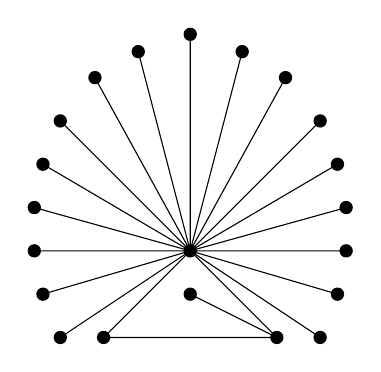
\begin{tikzpicture}[scale=1.1]
		\draw[fill=black] (-1,0) circle (2pt); \draw[fill=black] (1,0) circle (2pt); \draw[fill=black] (0,1) circle (2pt); \draw[fill=black] (0,.5) circle (2pt);
		\draw[thin] (-1,0)--(1,0)--(0,1)--(-1,0); \draw[thin] (1,0)--(0,.5);
		
		
		\draw[fill=black] (1.5,0) circle (2pt); \draw[fill=black] (1.7,.5) circle (2pt); \draw[fill=black] (1.8,1) circle (2pt); \draw[fill=black] (1.8,1.5) circle (2pt); \draw[fill=black] (1.7,2) circle (2pt); \draw[fill=black] (1.5,2.5) circle (2pt); \draw[fill=black] (1.1,3) circle (2pt); \draw[fill=black] (.6,3.3) circle (2pt); \draw[fill=black] (0,3.5) circle (2pt);
		
		\draw[thin] (1.7,.5)--(0,1)--(1.5,0); \draw[thin] (1.8,1)--(0,1)--(1.8,1.5); \draw[thin] (1.7,2)--(0,1)--(1.5,2.5); \draw[thin] (1.1,3)--(0,1)--(.6,3.3); \draw[thin] (-.6,3.3)--(0,1)--(0,3.5);
		
		
		\draw[fill=black] (-1.5,0) circle (2pt); \draw[fill=black] (-1.7,.5) circle (2pt); \draw[fill=black] (-1.8,1) circle (2pt); \draw[fill=black] (-1.8,1.5) circle (2pt); \draw[fill=black] (-1.7,2) circle (2pt); \draw[fill=black] (-1.5,2.5) circle (2pt); \draw[fill=black] (-1.1,3) circle (2pt); \draw[fill=black] (-.6,3.3) circle (2pt); 
		
		\draw[thin] (-1.7,.5)--(0,1)--(-1.5,0); \draw[thin] (-1.8,1)--(0,1)--(-1.8,1.5); \draw[thin] (-1.7,2)--(0,1)--(-1.5,2.5); \draw[thin] (0,1)--(-1.1,3); 
		
		
	\end{tikzpicture}
	\caption{Graph $G$ with $17$ pendent at one vertex of $K_{3}$, and one pendent at other vertex.}
	\label{unicyclic}
\end{figure}

Consider a graph  $G$ obtained form $K_{3}$ by attaching $a\geq 2$ number of pendents at one vertex and $1$ pendent at other vertex. The order of $G$ is $n=a+4.$ Let $u$ be the vertex of degree $a+2,$ $v$ be vertex of degree $3$, $w$ be vertex of degree $2$, $a_{i}$ be pendents for $1\leq i\leq a,$ $\{b\}$ be other pendent attached at $v$. Such a graph with $17$ pendent at one vertex of $K_{3}$, and one pendent at other vertex is shown in Figure \ref{unicyclic}.
With this vertex labelling, it follows that $\{a_{1},\dots,a_{a}\}$ is an independent set such that each $a_{i}$ share the same neighbor $u $. So, It is easy to see that  $0$ is the eigenvalue of $G$ with multiplicity at least $a-1,$ with eigenvectors $X_{i-1}=\big(0,0,0,0,1,x_{i2},x_{i3},\dots,x_{ia}\big)^{t}, 2\leq i \leq a$, where $x_{ij}=-1$ if $i=j$ and $0$, otherwise.
 The smallest equitable partition is $\{\{u\},\{v\},\{w\}, \{a_{1},\dots,a_{a}\},\{b\}\}$. With this partition, the adjacency matrix and its associated quotient matrix is 
 $$ A(G)=\left[ \begin{array}{c | c | c | c c c c | c}
	0 & 1 & 1 & 1 & 1 & \dots & 1 & 0 \\
	\hline
	1 & 0 & 1 & 0 & 0 & \dots & 0 & 1\\
	\hline
	1 & 1 & 0 & 0 & 0 &  \dots & 0 & 0\\
	\hline
	1 & 0 & 0 & 0 & 0 & \dots & 0 & 0\\
	\vdots & \vdots & \vdots & \vdots & \vdots & \ddots & \vdots & \vdots \\
	1 & 0 & 0 & 0 & 0 & \dots & 0 & 0\\
	1 & 0 & 0 & 0 & 0 & \dots & 0 & 0\\
	\hline
	0 & 1 & 0 & 0 & 0 & \dots & 0 & 0
\end{array}\right]\qquad \text{and}\qquad Q(G)=\begin{bmatrix}
	0 & 1 & 1 & a & 0\\
	1 & 0 & 1 & 0 & 1\\
	1 & 1 & 0 & 0 & 0\\
	1 & 0 & 0 & 0 & 0\\
	0 & 1 & 0 & 0 & 0
\end{bmatrix}. $$
The characteristic polynomial of $Q$ is $-x \left(x^{4}-(a+4) x^2-2 x+2 a+1\right).$ Therefore $Q$ contains all the $5$ distinct eigenvalues of $G$ with the smallest equitable partition (without enlarging any cell of partition). The other four eigenvalues of $A(G)$ cannot be precisely found. We illustrate it with the help of an example

Consider the case $a=2$. The adjacency and quotient matrices of  $G$ are 
$$ A(G)=\left[ \begin{array}{c | c | c | c c | c}
	0 & 1 & 1 & 1 & 1 & 0 \\
	\hline
	1 & 0 & 1 & 0 & 0 & 1\\
	\hline
	1 & 1 & 0 & 0 & 0 & 0\\
	\hline
	1 & 0 & 0 & 0 & 0 & 0\\
	1 & 0 & 0 & 0 & 0 & 0\\
	\hline
	0 & 1 & 0 & 0 & 0 & 0
\end{array}\right]\qquad\text{and}\qquad Q(G)=\begin{bmatrix}
	0 & 1 & 1 & 2 & 0\\
	1 & 0 & 1 & 0 & 1\\
	1 & 1 & 0 & 0 & 0\\
	1 & 0 & 0 & 0 & 0\\
	0 & 1 & 0 & 0 & 0
\end{bmatrix}. $$
The eigenvalues of $A(G)$ are $\{2.44579, 0.796815, 0^{2}, -1.37033, -1.87228\},$ and that of $Q$ are $\{2.44579,0.796815,0,-1.37033,-1.87228\}.$ We generalize this idea for weighted adjacency matrix. We recall the following definition.



The weighted adjacency matrix $\dot{A}(G)$ of a graph $G$ of order $n$ is a real symmetric matrix, which is defined as 
\begin{equation*}\label{general adjacency matrix}
	\dot{A}(G)=A_{\phi}(G)=(a_{\phi})_{n},\qquad \text{with}~ a_{ij}=\begin{cases}
		\phi(d_{u},d_{v}) & \text{if} ~ u\sim v\\
		0 & \text{otherwise},
	\end{cases}
\end{equation*}
where $u\sim v$ means adjacent relation. It is evident that the  matrix $\dot{A}(G)$ is a special type of weighted matrix with edge weights $w_{i,j}= \phi(d_{i},d_{j})$. Also note that $ w_{i,j}= \phi(d_{i},d_{j})= \phi(d_{j},d_{i})=w_{j,i}.$
The  matrix $\dot{A}(G)$ is the weighted matrix with edge weights based on vertex degrees in terms of symmetric function $w_{i,j}$. For $\phi(d_{i},d_{j})=1 $, we get the classical adjacent matrix $A(G)$, and for other values of $\phi(d_{i},d_{j})$, we obtain  the matrices like Zagreb Matrix, Sombor matrix, Geometric Arithmetic matrix, ABC matrix and many other matrices \cite{bilalmath}. 


Let $G$ obtained form $K_{3}$ by attaching $a\geq 2$ number of pendents at one vertex and $1$ pendent at other vertex. With partition $\{\{u\},\{v\},\{w\}, \{a_{1},\dots,a_{a}\},\{b\}\}$, the weighted matrix can be written as
$$ \dot{A}(G)=\begin{bmatrix}
	0 & \phi(a+2,3) & \phi(a+2,2) & \phi(a+2,1)J_{1\times a} & 0\\
	\phi(a+2,3) & 0 & \phi(3,2) & 0_{1\times a} & \phi(3,1)\\
	\phi(a+2,2) & \phi(3,2) & 0 & 0_{1\times a} & 0\\
	\phi(a+2,1)J_{a\times 1} & 0_{a\times 1} & 0_{a\times 1} & 0_{a} & 0_{a\times 1}\\
	0 & \phi(3,1) & 0 & 0_{1\times a} & 0
\end{bmatrix}, $$
where $0$ is a matrix of zeros and $J$ is a matrix of all ones. As above, $0$ is the eigenvalue of $\dot{A}(G)$ with multiplicity $a-1$, with same set of eigenvectors $X_{i-1}$ for $2\leq i\leq a$. The equitable quotient matrix is given as
 $$ Q(\dot{A}(G))=\left[
 \begin{array}{ccccc}
 	0 & \phi(a+2,3) & \phi(a+2,2) & a \phi(a+2,1) & 0 \\
 	\phi(a+2,3) & 0 & \phi(3,2) & 0 & \phi(3,1) \\
 	\phi(a+2,2) & \phi(3,2) & 0 & 0 & 0 \\
 	\phi(a+2,1) & 0 & 0 & 0 & 0 \\
 	0 & \phi(3,1) & 0 & 0 & 0 \\
 \end{array}
 \right]. $$
 The characteristic polynomial of $ Q(\dot{A}(G))$ is given as
 \begin{align*}
 	-x&\Big(x^{4}-x^2 \left(\phi(a+2,3)^2+\phi(a+2,2)^2+5 \phi(a+2,1)^2+\phi(3,2)^2+\phi(3,2)^2\right)\\
 	&-2 \phi(a+2,3) \phi(a+2,2) \phi(3,2) x+\phi(a+2,2)^2 \phi(3,2)^2+5 \phi(a+2,1)^2 \phi(3,2)^2\\
 	&+5 \phi(a+2,1)^2 \phi(3,2)^2\Big).
 \end{align*} Thus, $Q(\dot{A}(G))$ contains all the distinct eigenvalues of $ \dot{A}(G)$ with the smallest possible equitable partition $\{\{u\},\{v\},\{w\}, \{a_{1},\dots,a_{a}\},\{b\}\}$. We make it precise in the following result. 
 \begin{proposition}\label{rare graph unicyclic}
 	Let $G$ be a graph obtained form $K_{3}$ by attaching $a\geq 2$ number of pendents at one vertex and $1$ pendent at other vertex. Then the quotient matrix of $G$ contains all the distinct eigenvalues of the weighted adjacency matrix $\dot{A}(G)$ with the smallest equitable partition.
 \end{proposition}
 
 There may exist more classes of graphs with the property as in Proposition \ref{rare graph unicyclic}, but characterization of such a graphs is very important in the sense that from the smallest order quotient matrix  we get the information about the spectrum of the weighted adjacency matrix of a graph of arbitrary order $n.$
 
 Proposition \ref{rare graph unicyclic} cannot be extended to signless Laplacian matrix of $G$. As the signless Laplacian matrix of $G$ is 
 $$ S(G)=\begin{bmatrix}
 	a+2 & 1 & 1 & J_{1\times a} & 0\\
 	1 & 3 & 1 & 0_{1\times a} & 1\\
 	1 & 1 & 2 & 0_{1\times a} & 0\\
 	J_{a\times 1} & 0_{a\times 1} & 0_{a\times 1} & 0_{a} & 0_{a\times 1}\\
 	0 & 1 & 0 & 0_{1\times a} & 0
 \end{bmatrix}. $$
 It is easy to see that $S(G)$ has eigenvalue $1$ with multiplicity $a-1$, due to the presence of $a$ pendents sharing same neighbor. The equitable quotient matrix of $S(G)$ is
$$ Q(S(G))=\left[
 \begin{array}{ccccc}
 	a+2 & 1 & 1 & a & 0 \\
 	1 & 3 & 1 & 0 & 1 \\
 	1 & 1 & 2 & 0 & 0 \\
 	1 & 0 & 0 & 1 & 0 \\
 	0 & 1 & 0 & 0 & 1 
 \end{array} \right]. 
$$
The characteristic polynomial of $Q(S(G))$ is  
$$x^{5}-(a+9) x^4+(6 a+27) x^3-(9 a+35) x^2+(3 a+20) x-4. $$
So, the factor $x-1$ is missing in the above polynomial. Thus, the spectrum of $Q(S(G))$ does not contain all the distinct eigenvalues of $S(G).$ Similarly,  \ref{rare graph unicyclic} cannot be extended to distance and distance signless Laplacian matrices of $G.$ 
\begin{remark}\label{remark quotinet}
	If $G$ be a graph obtained form $K_{3}$ by attaching $a\geq 2$ number of pendents at one vertex and $1$ pendent at other vertex. Then the smallest equitable quotient matrix of $G$ with the smallest possible partition does not contain all the distinct eigenvalues of the signless Laplacian, distance and distance signless Laplacian matrices of $G.$
\end{remark}
We note that Remark \eqref{remark quotinet} is equally valid for weighted signless Laplacian matrices, like $ABC$ signless Laplacian matrix, Geometric Arithmetic signless Laplacian matrix, Sombor signless Laplacian matrix and other types of  weighted signless Laplacian matrices.
\section{Distinct eigenvalues of quotient matrices in terms of equitable partitions} \label{section 6}
Furthermore, Proposition \ref{rare graph unicyclic} has no meaning for the Laplacian matrix of a graph, as the row sum is always zero. So, the smallest equitable partition is itself $\{\{1,2,\dots,n\}\}$, and its associated quotient matrix is $(0)_{1\times 1} $, which contains only one eigenvalue $0$ of $G.$ As our graphs are non trivial, that are away from edgeless graphs, so we put our attention in the next second smallest equitable partition, such that the spectrum of the quotient matrix contains all the distinct eigenvalues of the Laplacian matrix of a graph $G.$



\begin{proposition}\label{rare graph unicyclic Laplacian}
	Let $G$ be a graph obtained form $K_{3}$ by attaching $a\geq 2$ number of pendents at one vertex and $1$ pendent at other vertex. Then the quotient matrix does not contains all the distinct eigenvalues of the Laplacian (distance Laplacian) matrix $G$ with the second smallest equitable partition $P=\{\{u\},\{v\},\{w\}, \{a_{1},\dots,a_{a}\},\{b\}\}.$
\end{proposition}
\begin{proof}
	We will work with the Laplacian matrix and same idea can be generalized to the distance Laplacian matrix of $G$ (or even other graph Laplacian matrices). The Laplacian matrix of $G$ is given as
	$$ L(G)=\begin{bmatrix}
		a+2 & -1 & -1 & -J_{1\times a} & 0\\
		-1 & 3 & -1 & 0_{1\times a} & -1\\
		-1 & -1 &  2 & 0_{1\times a} & 0\\
		-J_{a\times 1} &  0_{a\times 1}  & 0_{a\times 1} &  I_{a} & 0_{a \times 1}\\
		0 &  -1 & 0 & 0_{1\times a} & 1
	\end{bmatrix}, $$
	where $I_{a}$ is an identity matrix of order $a.$
	It is easy to verify that $1$ is the eigenvalue of $L(G)$ with multiplicity $a-1$. The other eigenvalues of $L(G)$ are the eigenvalues of the following equitable quotient matrix
	$$ Q(L(G))=\begin{bmatrix}
		a+2 & -1 & -1 & -a & 0\\
		-1 & 3 & -1 & 0 & -1\\
		-1 & -1 &  2 & 0 & 0\\
		-1 &  0  & 0 &  1 & 0\\
		0 &  -1 & 0 & 0 & 1
	\end{bmatrix}, $$
	its characteristic polynomial is $$x(x^{4}-(a+9) x^3+(6 a+27) x^2-(9 a+31) x+3 a+12). $$
	The above polynomial does not contain the eigenvalue $1$. Similarly, the eigenvalue $2a+8$ of the distance Laplacian matrix of $G$ is the not eigenvalue of the quotient matrix  with the second smallest equitable partition $P.$
\end{proof}

But in the generalized partition in which one cell is divided into two, we have the following result.
\begin{proposition}
	Let $M$ be the given in Proposition \ref{Qmat contains distinct eigenvalues of M}. Then the spectrum of its quotient matrix contains all the distinct eigenvalues of $M$ with the second smallest possible partition $P=\{\{1\},\{2\},\{3,\dots,n+2\}\}.$
\end{proposition}

\begin{remark}
	We are not sure, if $M$ given in Proposition \ref{Qmat contains distinct eigenvalues of M} is the distance Laplacian matrix of some graph, as it is a special case of the matrix (which is different from graph Laplacian matrix) given in Remark 2.9 \cite{bilalijpam}. But from the presentation of $M$, it looks some sort of Laplacian matrix.
\end{remark}

Let us look at the weak form of the Problem \ref{problem distinct 2}.
\begin{problem}\label{problem distinct 3}
	Characterize the classes of matrices such that the spectrum of the quotient matrix contains all the distinct eigenvalues of parent matrix with respect to the enlarged equitable partition (possibly smallest)?
\end{problem}
By Theorem \ref{theorem eqitable quotient matrix contains all the eigenvalues with some partition}, such a partition exits. And, we are asked  to search for second, third or so forth smallest equitable partition such that its equitable quotient matrix contains all the distinct eigenvalues of parent matrix. There may be more enlarged partitions but we are interested in the smallest possible enlarged partition which contains all the distinct eigenvalues of a parent matrix.
 Let us consider the quotient matrix given in Proposition \ref{rare graph unicyclic Laplacian}. As one eigenvalue is missing, so if we consider the enlarged partition $P=\{\{u\},\{v\},\{w\}, \{a_{1}\},\{a_{2},\dots,a_{a}\},\{b\}\}$, its portioned Laplacian matrix is 
$$ L(G)=\begin{bmatrix}
	a+2 & -1 & -1 & -1 &-J_{1\times (a-1)} & 0\\
	-1 & 3 & -1 & 0 & 0_{1\times (a-1)} & -1\\
	-1 & -1 &  2 & 0 & 0_{1\times (a-1)} & 0\\
	-1 & 0 & 0 & 1 & 0_{1\times (a-1)} & 0\\
	-J_{(a-1)\times 1} &  0_{(a-1)\times 1}  & 0_{(a-1)\times 1}  & 0_{(a-1)\times 1} &  I_{a-1} & 0_{(a-1) \times 1}\\
	0 &  -1 & 0 & 0 & 0_{1\times (a-1)} & 1
\end{bmatrix}. $$
The equitable quotient matrix of the above matrix $L(G)$ is 
$$ Q(L(G))=\begin{bmatrix}
	a+2 & -1 & -1 & -1 &-(a-1) & 0\\
	-1 & 3 & -1 & 0 & 0 & -1\\
	-1 & -1 &  2 & 0 & 0 & 0\\
	-1 & 0 & 0 & 1 & 0 & 0\\
	-1 &  0  & 0  & 0 &  1 & 0\\
	0 &  -1 & 0 & 0 & 0 & 1
\end{bmatrix}. $$
The characteristic polynomial  of $Q(L(G))$ is
$$ x(x-1)\left(x^{4}-(a+9) x^3+(6 a+27) x^2-(9 a+31) x+3 a+12\right).$$
The above polynomial contains all the distinct eigenvalues of  $L(G)$ with enlarged partition $P=\{\{u\},\{v\},\{w\},\{a_{1}\},\{a_{2},\dots,a_{a}\},\{b\}\}.$ Thus, $Q(L(G))$ contains all the distinct eigenvalues of $L(G)$ with the smallest enlarged partition. We note that such a partition is not unique as the vertex set $\{a_{1},a_{2},\dots,a_{a}\}$ can be enlarged in $\binom{a}{1}=a$ ways. A similar idea of partition works for the distance Laplacian matrix of a graph $G.$

\vskip 2mm
We now turn our attention to Problem \ref{problem distinct 3}, and work for graph matrices with special features.

If $G$ be a graph of order $n$ with independent set $S=\{v_{1},v_{2},\dots,v_{\alpha}\}. $ If $a> \frac{n}{2}$, then there are at least two pendent vertices $\{v_{1},v_{2}\}$ share the same neighbors. If each vertex of $S$ have the same number of neighbors, then $ \beta$ is the eigenvalue of some graph matrix. As in this case the row sum corresponding to vertices of $S$ is constant of  graph matrix $M(G).$ Choosing eigenvectors with zero entries on remaining vertices and $1$ at $v_{1}$-th coordinate, and rotating $-1$ for exactly one $v_{i}$ $(2\leq i\leq \alpha)$, and putting other coordinates of $v_{j}$ as zero. We obtain $\alpha-1$ eigenvectors related to eigenvalue $\beta$ of $M(G).$ The eigenvalue $\beta$ may or may not be the eigenvalue of the quotient matrix with respect to the smallest equitable partition. But, however if we decompose $S$ as $S=\{v_{i}\}\cup \{v_{1},\dots,v_{i-1},v_{i+1},\dots,v_{\alpha}\},$ then with the new enlarged partition $\{C_{1},\dots,C_{\eta}, \{i\},\{1,2,\dots,i-1,i+1,\dots,\alpha\}\}$, the equitable quotient matrix will contain all the missing eigenvalue $\beta$ of $M(G),$
where  $C_{i}$ are other partition cells. If $M(G)$ is a weighted adjacency matrix, and if there are more independent sets like $S_{i}$ with same properties as with $S,$ then it is enough to enlarge just one $S_{i}$, otherwise it will lead to repeated multiplicity of the eigenvalue $\beta.$ For Laplacian (signless) or distance based Laplacian (signless) matrices, the transmission may be different and different independent may lead to different eigenvalues $\beta_{i}$ with multiplicity $|S_{i}|-1$. In this case, we divide each cell corresponding to $S_{i}$ as $\{\{j\},\{1,2,\dots,j-1,j+1,\dots,|S_{i}|\}\}$ and the equitable quotient will contain all the missing eigenvalues $\beta_{i}$ of graph matrix $M(G)$ with this new enlarged partition. If $\alpha\leq \frac{n}{2},$ then there may exist independent sets  $S$ with cardinality $\alpha$, such that no two vertices share the same neighbours. In this cases, $\beta$ may not be an eigenvalue of $M(G)$. Though, if $\alpha>\frac{n}{2},$ then at least two vertices in $G$ share the same neighbors, and $\beta$ is the eigenvalue of $M(G).$ Now, enlarged the partition cell as above, and we can find $\beta$ in the smallest possible enlarged quotient matrix.  If $S$ is a clique and each vertex of $S$ share the same numbers of neighbors outside $S$, then $\gamma$ is the eigenvalue of graph $M(G)$ with multiplicity $|S|-1$. With a similar idea of the partition decomposition as in independent case, we get an enlarged partition with new partition cells $ \{i\},\{1,2,\dots,i-1,i+1,\dots,\alpha\}$, such that the quotient matrix contains the eigenvalue $\gamma.$ We make these observations, precise in the following result.
\begin{theorem}\label{end}
	If $G$ is a graph of order $n,$ and $M(G)$ is its graph matrix. Then the following hold.
	\begin{enumerate}
		\item If $ S=\{v_{1}, v_{2},\dots, v_{\alpha}\} $ be an independent subset of $ G $ such that $ N(v_{i})=N(v_{j})$, for all $ i,j\in \{1,2,\dots,\alpha \} $, and $\beta$ is an eigenvalue of $M(G)$. Then the quotient matrix of enlarged partition with cells $\{\{i\}, \{1,\dots,i-1,i+1, \alpha\}\}$ contains the eigenvalue of $\beta$ of $M(G).$
	\item  If $ S=\{v_{1}, \dots, v_{\alpha}\} $ be a clique of $ G $ such that $ N(v_{i}) \setminus \{v_{j}\}=N(v_{j})\setminus \{v_{i}\}$, for all $ i,j\in \{1,\dots,\alpha \} $, and $\gamma$ is an eigenvalue of $M(G)$. Then the quotient matrix of enlarged partition with cells $\{\{i\}, \{1,\dots,i-1,i+1, \alpha\}\}$ contains the eigenvalue of $\gamma$ of $M(G).$
	\end{enumerate}
\end{theorem}

Consider the complete bipartite graph $K_{a,b}, a\neq b$ and $A(K_{a,b})$ be its adjacency matrix. Then $A(K_{a,b})=\begin{bmatrix}
0_{a} &J_{a\times b}\\
J_{b\times a} & 0_{b}
\end{bmatrix}.$ With partition $p=\{\{1,2,\dots,a\},\{1,2,\dots,b\}\}$, the equitable quotient matrix is $ Q(K_{a,b})=\begin{bmatrix}
0 & b\\ a & 0
\end{bmatrix},$ and its eigenvalues are $\pm \sqrt{ab}$. However, it has two independent sets, and each vertex in one set is sharing the same number of neighbours. Also, the eigenvalue $0$ is missing in the smallest equitable quotient matrix. By above theorem and its observations, we can break any of these two independent sets and enlarge the partition like $P=\{\{1\},\{2,\dots,a\},\{1,2,\dots,b\}\}.$ The equitable quotient matrix with this partition is $Q^{\prime}=\begin{bmatrix}
0 & 0 & b\\
0 & 0 & b\\
1 & a-1 & 0
\end{bmatrix},$ and its spectrum is $\{0,\pm\sqrt{ab}\}.$ Thus, $Q^{\prime}$ contains all the distinct eigenvalues of $ A(K_{a,b}).$ For the Laplacian matrix of $K_{a,b}$, we have $L(K_{a,b})=\begin{bmatrix}
bI_{a} & -J_{a\times b}\\
-J_{b\times a} & aI_{b}
\end{bmatrix},$ and its smallest equitable quotient matrix is $Q(L(K_{a,b}))=\begin{bmatrix}
b & -b\\ -a & a
\end{bmatrix}.$ The spectrum of $ Q(L(K_{a,b}))$ is $\{0,a+b\}$ with partition is $\{\{1,2,\dots,a\},\{1,2,\dots,b\}\}$. Due to different degrees for two independent sets of $K_{a,b},$ we enlarged one by one partition cells $\{1,2,\dots,a\}$ and $\{1,2,\dots,b\}$, or both of them together. So, quotient matrix with equitable partition $P=\{\{1\},\{2,\dots,a\},\{1\},\{2,\dots,b\}\}$ is 
$$ Q(L(K_{a,b}))=\left[
\begin{array}{cccc}
	b & 0 & -1 & -(b-1) \\
	0 & b & -1 & -(b-1) \\
	-1 & -(a-1) & a & 0 \\
	-1 & -(a-1) & 0 & a \\
\end{array}
\right], $$
and its eigenvalues are $\{0,a,b,a+b\}.$ Thus, the quotient matrix with enlarged partition $P $ contains all the distinct eigenvalues of $ L(K_{a,b}).$ Let $G\cong CS(\omega,\alpha)$ be a complete split graph with clique number $\omega$ and independence number $\alpha$. The distance signless Laplacian matrix of $ G$ is $D^{Q}(G)=\begin{bmatrix} (\omega+\alpha-2)I_{\omega}+J_{\omega}& J_{\omega\times \alpha}\\ J_{\alpha\times \omega} & (\omega+2\alpha-4)I_{\alpha}+2J_{\alpha}
\end{bmatrix}.$ The equitable quotient matrix with partition is $\{\{1,2,\dots,\omega\},\{1,2,\dots,\alpha\}\}$ is $Q(D^{Q}(G))=\left[ \begin{array}{cc}
a+2 w-2 & a \\
w & 4 a+w-4 
\end{array}
\right],$ and its eigenvalues are $\frac{1}{2} \left(5 \alpha+3 \omega-6\pm \sqrt{9 \alpha^2-2 \alpha \omega-12 \alpha+\omega^2+4 \omega+4}\right)$. Now, enlarging the clique cell $\{1,2,\dots,\omega\}$ and the independent cell $\{1,2,\dots,\alpha\}$, and consider the quotient matrix of new partition $P^{\prime}=\{\{1\},\{2,\dots,\omega\},\{1\},\{2,\dots,\alpha\}\}$, we have
$$ Q^{\prime}(D^{Q}(G))=\left[
\begin{array}{cccc}
	\alpha+\omega-1 & \omega-1 & 1 & \alpha-1 \\
	1 & \alpha+2 \omega-3 & 1 & \alpha-1 \\
	1 & \omega-1 & 2 (\alpha-1)+\omega & 2 (\alpha-1) \\
	1 & \omega-1 & 2 & 4 \alpha+\omega-6 \\
\end{array}
\right].$$
The eigenvalues of the above matrix are 
$$ \Big\{\alpha + \omega-2, 2 \alpha + \omega-4,  \frac{1}{2} \left(5 \alpha+3 \omega-6\pm \sqrt{9 \alpha^2-2 \alpha \omega-12 \alpha+\omega^2+4 \omega+4}\right)\Big\}. $$
That illustrates the application of Theorem \ref{end} for both cases of clique and an independent sets for the distance Laplacian matrix. Thus, with the enlarged partition $P^{\prime}$, the equitable quotient matrix $Q^{\prime}$ contains all the distinct eigenvalues of the complete split graph.

The Problem \ref{problem distinct 3} remains open in general for large classes of graph matrices. When spectrum of a graph matrix $M(G)$ is symmetric towards its origin, then we need to divide two partition cells simultaneously. 

\section{Conclusion}

In this paper, we have investigated when the spectral information of a square matrix $M$ can be faithfully recovered from an equitable quotient matrix $Q$ arising from a partition of its index set. Starting from the notion of an equitable partition, we identified broad classes of matrices for which the equitable quotient matrix contains all distinct eigenvalues of $M$. In these cases, the (possibly much smaller) matrix $Q$ completely encodes the distinct eigenvalues of the parent matrix $M$, and hence provides a substantial reduction in dimension without any loss of spectral information at the level of distinct eigenvalues (Theorem \ref{thm:n-by-n-two-eigs}).

A central contribution of our work is the derivation of necessary and sufficient conditions for a distinct eigenvalue of $M$ to appear in the spectrum of $Q$ in terms of the eigenspaces of $M$ and the structure of the partition (Theorem \ref{thm:equitable-all-eigs-general}). These conditions clarify how the choice of partition interacts with the geometry of eigenspaces, and they characterize precisely when an equitable quotient captures a given eigenvalue. 

We have also explored applications of these ideas in the context of graph matrices, where $M$ arises from a natural matrix associated with a graph, and the partition is induced by a structural decomposition such as vertex classes or symmetry orbits. In this setting, we showed that a suitable (and sometimes slightly enlarged) equitable partition allows one to read off the distinct eigenvalues of the parent matrix from the corresponding quotient matrix (Proposition \ref{rare graph unicyclic} and Theorem \ref{end}). This leads to efficient ways of obtaining spectral information for large graphs by working with comparatively small quotient matrices.   Possible directions for future work include extending these techniques to broader classes of matrices and partitions (for example, almost equitable partitions), studying stability under perturbations of $M$ and of the partition, and further exploiting these ideas in algorithmic applications where one needs to approximate or track eigenvalues of large structured matrices.

\section*{Declarations}
\noindent \textbf{Data Availability:}	There is no data associated with this article as data sharing is not applicable since no data sets were generated or analyzed during the current study.

\noindent \textbf{Funding:} The authors declare that no funds, grants, or other support were received during the preparation of this manuscript.

\noindent \textbf{Conflict of interest:} The authors have no competing interests to declare that are relevant to the content of this article.

\noindent\textbf{Note:} I welcome any comments and suggestions regarding this article; please feel free to contact me at \href{bilalahmadrr@gmail.com}{bilalahmadrr@gmail.com}



\begin{thebibliography}{0}

\bibitem{atik}	F. Atik, On equitable partition of matrices and its applications, \emph{Linear Multilinear Algebra} \textbf{68}(11) (2020) 2143--2156.
\bibitem{atikELA2018}  {F. Atik and P. Panighari, On the distance and distance signless Laplacian eigenvalues of graphs and the smallest Gre\v{s}gorin disc, \em Electronic J. Linear Algebra} {\bf 34} (2018) 191--204.
%\bibitem{AH1} M. Aouchiche and  P. Hansen,  Distance spectra of graphs: a survey,  \textit{Linear Algebra Appl.} {\bf 458} (2014) 301--386.
%\bibitem{AH2} M. Aouchiche and  P. Hansen,  Two Laplacians for the distance matrix of a graph, \textit{Linear Algebra Appl.} {\bf 439} (2013) 21--33.
%\bibitem{AH3} M. Aouchiche and  P. Hansen,  Some properties of the distance Laplacian eigenvalues a graph,  \textit{Czech. Math. J.} {\bf 64,139} (2014) 751--761.

\bibitem{BH} A. E. Brouwer and W. H. Haemers, \textit{Spectra of Graphs}, Springer, New York, 2010.
%\bibitem{sc} {S. Chattopadhyay, K. L. Patra and B. K. Sahoo, Laplacian eigenvalues of the zero divisor graph of the ring $ \mathbb{Z}_{n} $, \em Linear Algebra Appl.} {\bf 584} (2020) 267--286.
\bibitem{cds} D. M. Cvetkovi\'{c}, P. Rowlison and S. Simi\'c, \textit{An Introduction to Theory of Graph Spectra}, London Math. Society Student Text, 75, Cambridge University Press, UK, 2010.
%\bibitem{dah} {K. C. Das,  M. Aouchiche and P. Hansen, On (distance) Laplacian energy and (distance) signless Laplacian energy of graphs, \textit{Discrete Appl. Math.}} {\bf 243} (2018) 172--185.
%\bibitem{dr} {R. C. Diaz and O. Rojo, Sharp upper bounds on the distance energies of a graph, \textit{ Linear Algebra Appl.}} {\bf 545} (2018) 55--75.
\bibitem{vilmar} E. Fritscher, and V. Trevisan, Exploring symmetries to decompose matrices and graphs preserving the spectrum, \textit{SIAM J. Matrix Analysis  Appl.} \textbf{37}(1) (2016) 260--289.
\bibitem{hjl} S. R. Garcia and R. A. Horn, \emph{A Second Course in Linear Algebra}, Cambridge University Press, UK, 2017.
%\bibitem{hilal2020} H. A. Ganie, On distance Laplacian spectrum (energy) of graphs,  \textit{Discrete Math. Algorithms Appl.} (2020) 2050061 DOI:10.1142/S1793830920500615.
%\bibitem{hilal2021} H. A. Ganie, On the distance Laplacian energy ordering of trees, \emph{Applied Math. Computation} \textbf{394} (2021) 125762.
\bibitem{heamers} W. H. Haemers, Interlacing eigenvalues and graphs, \textit{Linear Algebra Appl.} {\bf 226-288} (1995) 593--616.
\bibitem{hj} R. Horn and C. Johnson,  \textit{Matrix Analysis}, Second Edition, Cambridge University Press, New York, (2013).
\bibitem{mehreen1} Z. Mehranian, A. Gholami and A. R. Ashrafi, The spectra of power graphs of certain finite groups,  Linear Multilinear Algebra  {\bf 65}(5) (2016) 1003--1010.

%\bibitem{pbt} S. Pirzada, Bilal A. Rather and T. A. Chishti, On distance Laplacian spectrum of zero divisor graphs of $\mathbb{Z}_{n}$, {\it Carpathian Mathematical Publications}, \textbf{13(1)} (2021) 48--57. 
%\bibitem{pbrm}   S. Pirzada, Bilal A. Rather, R. Ul Shaban, Merajuddin, On signless Laplacian spectrum of the zero divisor graph of the ring $\mathbb{Z}_{n}$, {\it Korean J. Math.} {\bf 29,1} 13-24.
\bibitem{bilal2020}	S. Pirzada, B. A. Rather, M. Aijaz and T. A. Chishti, Distance signless Laplacian spectrum of graphs and spectrum of zero divisor graphs of  $ \mathbb{Z}_{n}, $  \emph{Linear MultiLinear Algebra} \textbf{70}(17) (2022) 3354--3369.
\bibitem{bilalmath} B. A. Rather, H. A. Ganie, K. C. Das and Y. Shang, General extended adjacency eigenvalues of chain graphs,  \emph{Math.} \textbf{12}(2) (2024) 192.
\bibitem{bilalijpam} B. A. Rather, A note on the distinct eigenvalues of quotient matrices, \textit{Indian J. Pure Appl. Math.} \textbf{55} (2024) 1429--1439.
\bibitem{bilallapsurvey} B. A. Rather and M. Aouchiche, Distance Laplacian spectra of graphs: a survey, \emph{Discrete Appl. Math.} \textbf{361} (2025) 136--195.
\bibitem{bilalslapsurvey} B. A. Rather, H. A. Ganie, and J. Wang, Distance signless Laplacian spectra of graphs: a survey, \emph{Discrete Appl. Math.} (2025), in press.
\bibitem{bilal}  B. A. Rather, S. Pirzada and Z. Goufei, On distance Laplacian spectra of power graphs of certain finite groups, \emph{Acta Math. Sinica, English Series} \textbf{39} (2023) 603--617.
%\bibitem{torktaz} M. Torktaz and A. R. Ashrafi, Spectral properties of the commutating graphs of certain finite groups, \emph{AKCE Int. J. Graphs and Combinatorics}, \textbf{16} (2019) 300--309.
\bibitem{DS} D. Stevanovi\'{c},  Large sets of long distance equienergetic graphs,  \textit{Ars Math. Contemp.} {\bf 2}(1) (2009) 35--40.
\bibitem{you} {L. You, M. Yang, W. So and W. Xi, On the spectrum of an equitable quotient matrix and its applications, \textit{Linear Algebra Appl.}} {\bf 577} (2019) 21--40.

\end{thebibliography}


\end{document} 
